% Options for packages loaded elsewhere
\PassOptionsToPackage{unicode}{hyperref}
\PassOptionsToPackage{hyphens}{url}
\PassOptionsToPackage{dvipsnames,svgnames,x11names}{xcolor}
%
\documentclass[
  12pt,
  letterpaper,
  egregdoesnotlikesansseriftitles]{scrreprt}

\usepackage{amsmath,amssymb}
\usepackage{iftex}
\ifPDFTeX
  \usepackage[T1]{fontenc}
  \usepackage[utf8]{inputenc}
  \usepackage{textcomp} % provide euro and other symbols
\else % if luatex or xetex
  \usepackage{unicode-math}
  \defaultfontfeatures{Scale=MatchLowercase}
  \defaultfontfeatures[\rmfamily]{Ligatures=TeX,Scale=1}
\fi
\usepackage{lmodern}
\ifPDFTeX\else  
    % xetex/luatex font selection
  \setmainfont[]{Palatino Linotype}
\fi
% Use upquote if available, for straight quotes in verbatim environments
\IfFileExists{upquote.sty}{\usepackage{upquote}}{}
\IfFileExists{microtype.sty}{% use microtype if available
  \usepackage[]{microtype}
  \UseMicrotypeSet[protrusion]{basicmath} % disable protrusion for tt fonts
}{}
\makeatletter
\@ifundefined{KOMAClassName}{% if non-KOMA class
  \IfFileExists{parskip.sty}{%
    \usepackage{parskip}
  }{% else
    \setlength{\parindent}{0pt}
    \setlength{\parskip}{6pt plus 2pt minus 1pt}}
}{% if KOMA class
  \KOMAoptions{parskip=half}}
\makeatother
\usepackage{xcolor}
\setlength{\emergencystretch}{3em} % prevent overfull lines
\setcounter{secnumdepth}{5}
% Make \paragraph and \subparagraph free-standing
\ifx\paragraph\undefined\else
  \let\oldparagraph\paragraph
  \renewcommand{\paragraph}[1]{\oldparagraph{#1}\mbox{}}
\fi
\ifx\subparagraph\undefined\else
  \let\oldsubparagraph\subparagraph
  \renewcommand{\subparagraph}[1]{\oldsubparagraph{#1}\mbox{}}
\fi


\providecommand{\tightlist}{%
  \setlength{\itemsep}{0pt}\setlength{\parskip}{0pt}}\usepackage{longtable,booktabs,array}
\usepackage{calc} % for calculating minipage widths
% Correct order of tables after \paragraph or \subparagraph
\usepackage{etoolbox}
\makeatletter
\patchcmd\longtable{\par}{\if@noskipsec\mbox{}\fi\par}{}{}
\makeatother
% Allow footnotes in longtable head/foot
\IfFileExists{footnotehyper.sty}{\usepackage{footnotehyper}}{\usepackage{footnote}}
\makesavenoteenv{longtable}
\usepackage{graphicx}
\makeatletter
\def\maxwidth{\ifdim\Gin@nat@width>\linewidth\linewidth\else\Gin@nat@width\fi}
\def\maxheight{\ifdim\Gin@nat@height>\textheight\textheight\else\Gin@nat@height\fi}
\makeatother
% Scale images if necessary, so that they will not overflow the page
% margins by default, and it is still possible to overwrite the defaults
% using explicit options in \includegraphics[width, height, ...]{}
\setkeys{Gin}{width=\maxwidth,height=\maxheight,keepaspectratio}
% Set default figure placement to htbp
\makeatletter
\def\fps@figure{htbp}
\makeatother
\newlength{\cslhangindent}
\setlength{\cslhangindent}{1.5em}
\newlength{\csllabelwidth}
\setlength{\csllabelwidth}{3em}
\newlength{\cslentryspacingunit} % times entry-spacing
\setlength{\cslentryspacingunit}{\parskip}
\newenvironment{CSLReferences}[2] % #1 hanging-ident, #2 entry spacing
 {% don't indent paragraphs
  \setlength{\parindent}{0pt}
  % turn on hanging indent if param 1 is 1
  \ifodd #1
  \let\oldpar\par
  \def\par{\hangindent=\cslhangindent\oldpar}
  \fi
  % set entry spacing
  \setlength{\parskip}{#2\cslentryspacingunit}
 }%
 {}
\usepackage{calc}
\newcommand{\CSLBlock}[1]{#1\hfill\break}
\newcommand{\CSLLeftMargin}[1]{\parbox[t]{\csllabelwidth}{#1}}
\newcommand{\CSLRightInline}[1]{\parbox[t]{\linewidth - \csllabelwidth}{#1}\break}
\newcommand{\CSLIndent}[1]{\hspace{\cslhangindent}#1}


% Wird für die Tabelle im Titelblatt der Experten verwendet:
% Array
\usepackage{array}
% Neue Definition für Tabelleneinträge
% linksbündig mit Breitenangabe
\newcolumntype{L}[1]{>{\raggedright\arraybackslash}p{#1}} 
% zentriert mit Breitenangabe
\newcolumntype{C}[1]{>{\centering\arraybackslash}p{#1}} 
% rechtsbündig mit Breitenangabe
\newcolumntype{R}[1]{>{\raggedleft\arraybackslash}p{#1}} 

\usepackage[a4paper, margin=3cm]{geometry}

% Change math font





\makeatletter
\makeatother
\makeatletter
\@ifpackageloaded{bookmark}{}{\usepackage{bookmark}}
\makeatother
\makeatletter
\@ifpackageloaded{caption}{}{\usepackage{caption}}
\AtBeginDocument{%
\ifdefined\contentsname
  \renewcommand*\contentsname{Inhaltsverzeichnis}
\else
  \newcommand\contentsname{Inhaltsverzeichnis}
\fi
\ifdefined\listfigurename
  \renewcommand*\listfigurename{Abbildungsverzeichnis}
\else
  \newcommand\listfigurename{Abbildungsverzeichnis}
\fi
\ifdefined\listtablename
  \renewcommand*\listtablename{Tabellenverzeichnis}
\else
  \newcommand\listtablename{Tabellenverzeichnis}
\fi
\ifdefined\figurename
  \renewcommand*\figurename{Abbildung}
\else
  \newcommand\figurename{Abbildung}
\fi
\ifdefined\tablename
  \renewcommand*\tablename{Tabelle}
\else
  \newcommand\tablename{Tabelle}
\fi
}
\@ifpackageloaded{float}{}{\usepackage{float}}
\floatstyle{ruled}
\@ifundefined{c@chapter}{\newfloat{codelisting}{h}{lop}}{\newfloat{codelisting}{h}{lop}[chapter]}
\floatname{codelisting}{Listing}
\newcommand*\listoflistings{\listof{codelisting}{Listingverzeichnis}}
\makeatother
\makeatletter
\@ifpackageloaded{caption}{}{\usepackage{caption}}
\@ifpackageloaded{subcaption}{}{\usepackage{subcaption}}
\makeatother
\makeatletter
\@ifpackageloaded{tcolorbox}{}{\usepackage[skins,breakable]{tcolorbox}}
\makeatother
\makeatletter
\@ifundefined{shadecolor}{\definecolor{shadecolor}{rgb}{.97, .97, .97}}
\makeatother
\makeatletter
\makeatother
\makeatletter
\makeatother
\ifLuaTeX
\usepackage[bidi=basic]{babel}
\else
\usepackage[bidi=default]{babel}
\fi
\babelprovide[main,import]{ngerman}
% get rid of language-specific shorthands (see #6817):
\let\LanguageShortHands\languageshorthands
\def\languageshorthands#1{}
\ifLuaTeX
  \usepackage{selnolig}  % disable illegal ligatures
\fi
\IfFileExists{bookmark.sty}{\usepackage{bookmark}}{\usepackage{hyperref}}
\IfFileExists{xurl.sty}{\usepackage{xurl}}{} % add URL line breaks if available
\urlstyle{same} % disable monospaced font for URLs
\hypersetup{
  pdftitle={Tragverhalten von Stahlbetontragwerken},
  pdfauthor={Pascal Gitz},
  pdflang={de},
  colorlinks=true,
  linkcolor={Black},
  filecolor={Maroon},
  citecolor={Blue},
  urlcolor={Blue},
  pdfcreator={LaTeX via pandoc}}

% TITELBLATT, VERSIONSTABELLE UND SELBSTSTÄNDIGKEITSERKLÄRUNG
%--------------------------------------------------------------------------------------------------------------------


\titlehead{\includegraphics[height=0.5cm]{../images/logos/logo-mse}\hfill\includegraphics[height=0.5cm]{../images/logos/logo-hslu-en-col} \\ }
\subject{MASTER OF SCIENCE IN ENGINEERING\\Vertiefungsmodul I}
\title{Tragverhalten von Stahlbetontragwerken}

\subtitle
{Ansätze zur Verformungsberechnung}

%\thanks{
%Version 1.0
%\hfill \today
%\hfill Hun}


\date{\large Horw, Freitag, 19. Januar 2024}
\author{Pascal Gitz}

\publishers{
	\begin{table}[H]
		\centering
		\begin{tabular}{L{2cm} L{6cm}}
			Advisor: & Prof. FH, Dr. Daniel Heinzmann \\
			Experte: & Dr. Thomas Jäger \\
		\end{tabular}
	\end{table}
}
\begin{document}
\maketitle

Hiermit erkläre ich, dass ich die vorliegende Arbeit selbstständig angefertigt und keine anderen als die angegebenen Hilfsmittel verwendet habe. Sämtliche verwendeten Textausschnitte, Zitate oder Inhalte anderer Verfasser wurden ausdrücklich als solche gekennzeichnet.\\%
%
\\%
%
Horw, 21. Januar 2023 \hfill Pascal Gitz%

\vfill
%\begin{tabular}[h]{llcr} 
    %*Version 2.0 & - Definitives Exemplar & \today & MK \\ 
    %*Version 1.0 & - Prüfungsexemplar & 22. Januar 2021 & MK \\ 
%\end{tabular}\\

% Version 2.0 - Definitives Exemplar \hfill \today \quad \quad \quad \quad \quad MK\\
% Version 1.0 - Prüfungsexemplar \hfill 19. Januar 2023 \quad \quad \quad \quad \quad PG\\
Version 0.9 - Entwurf \hfill 08. Januar 2023 \quad \quad \quad \quad \quad PG\\

\newpage

\chapter*{Kurzfassung}

Die vorliegende Arbeit befasst sich mit Verformungen im Stahlbetonbau. Speziell mit den Verformungen von Stabtragwerken. Dazu sind unterschiedliche Modelle zur rechnerischen Bestimmung aufgezeigt. Als übergeordnetes Ziel gilt es praxistaugliche Berechnungsmethoden zu verwenden. Dies bedeutet möglichst geringen Berechnungsaufwand bei gleichzeitig hoher Genauigkeit.  

Das einleitende Kapitel beschreibt die Hintergründe der Modelle. Es wird auf das Modell des reinen Biegeträgers, die Methode der Mohr'schen Analogie, eine Abschätzung nach der Schweizerischen Betonnorm, das Zuggurtmodell, eine Integrationsmethode zur Berücksichtigung einer nicht-linearen Momenten-Krümmungs-Beziehung, sowie abschliessend auf eine Fachwerksanalyse eingegangen. Neben den theoretischen Grundlagen zeigt dir Arbeit die Anwendung der Modelle an einem Dreipunktbiegeversuch und einem Vierpunktbiegeversuch. Die Versuchsanwendung wird jeweils mit einer ausführlichen Diskussion der Ergebnisse abgeschlossen, verifiziert an den gemessenen Versuchsdaten. 

Der Modellvergleich zeigt, dass mit Berechnungsmethoden mit konstanten Biegesteifigkeiten, wie in der Praxis üblich, Verformungen nur bedingt präzise berechnet werden können. Die Verwendung von einer nicht-linearen Momenten-Krümmungs-Beziehungen ist für die Nachrechnung der Verformungen von Versuchen, belastet bis zum Versagen, unerlässlich. Die Fachwerksanalyse liefert bei beiden Versuchen die treffendsten Ergebnisse, sofern die Fachwerkshöhe exakt bestimmt werden kann. 


Im abschliessenden Kapitel wird das Ziel beschrieben, in einer folgenden Arbeit, die aufgezeigten Modelle auf Plattentragwerke zu erweitern. Als Ansatz dazu soll die Modellierung als Trägerrost dienen.

\ifdefined\Shaded\renewenvironment{Shaded}{\begin{tcolorbox}[enhanced, interior hidden, sharp corners, boxrule=0pt, borderline west={3pt}{0pt}{shadecolor}, breakable, frame hidden]}{\end{tcolorbox}}\fi

\renewcommand*\contentsname{Inhaltsverzeichnis}
{
\hypersetup{linkcolor=}
\setcounter{tocdepth}{1}
\tableofcontents
}
\listoffigures
\listoftables
\bookmarksetup{startatroot}

\hypertarget{einleitung}{%
\chapter{Einleitung}\label{einleitung}}

Bei der Analyse des Tragverhaltens ist die Bestimmung von Verformungen
im Stahlbetonbau in der Praxis oftmals mit Unsicherheiten verbunden. Die
vorwiegend aus Biegung resultierenden Verformungen werden unter der
Annahme einer konstanten Biegesteifigkeit berechnet. Diese wird
grundsätzlich am gerissenen oder am ungerissenen Querschnitt bestimmt.
Mit dieser Arbeit sollen die Grenzen dieser Modellvorstellung aufgezeigt
werden. Des Weiteren wird versucht, mit einem möglichst pragmatischen
Ansatz die eingeschränkte Modellvorstellung zu erweitern und die
Verformungen präzise abzubilden.

Die Arbeit umfasst ein einleitendes Kapitel, welches die Modelle in
ihren Grundeigenschaften aufgreift und erläutert, gefolgt von zwei
Kapiteln, welche die Anwendung der Modelle aufzeigen. Es wird ein
Dreipunktbiegeversuch aus dem Versuchsbericht
{[}\protect\hyperlink{ref-Jaeger2006}{1}{]}, sowie ein
Vierpunktbiegeversuch aus dem Versuchsbericht
{[}\protect\hyperlink{ref-Tue2019}{2}{]} analysiert. Es werden
ausschliesslich Stabtragwerke betrachtet. Das Berechnungsvorgehen ist
für beide Versuche analog zueinander. Die Kapitel werden mit einem
Modellvergleich abgeschlossen. Der Schlusspunkt der Arbeit liefert ein
Fazit, welches die Erkenntnisse der Berechnungen erneut aufgreift,
zusammenfasst und interpretiert.

Abschliessend lässt sich festhalten, dass diese Arbeit das grundlegende
Verständnis der Verformungen im Stahlbetonbau schärfen soll. Dazu sollen
Methoden aufgezeigt werden, durch welche sich die Verformungen
rechnerisch ermitteln lassen. Stets im Sinne der praktischen Anwendung.

\bookmarksetup{startatroot}

\hypertarget{sec-modellbeschrieb}{%
\chapter{Modellbeschreibung}\label{sec-modellbeschrieb}}

In diesem Kapitel sind Modelle zur Bestimmung von Verformungen im
Stahlbeton aufgezeigt. Es wird auf analytische Beziehungen und deren
Herleitungen eingegangen. Das Ziel ist es, die grundlegenden
Eigenschaften der Modelle darzulegen.

\hypertarget{sec-kontinua}{%
\section{Reiner Biegeträger}\label{sec-kontinua}}

Das Modell des reinen Biegeträgers ermöglicht die Ermittlung sämtlicher
Zustandslinien der Schnittgrössen basierend auf differentiellen
Beziehungen.

\begin{quote}
\emph{Die Verknüpfung der Gleichgewichtsbedingungen mit den
kinematischen Relationen, sowie den linear elastischen Stoffgleichungen
führt auf gewöhnliche Differentialgleichungen für die je nach
Problemstellung relevanten Verschiebungsgrössen, und aus diesen ergeben
sich die interessierenden inneren Verformungs- und Kraftgrössen in
Abhängigkeit der Lage auf der Stabachse.} Beschreibt
{[}\protect\hyperlink{ref-Marti}{3}{]} in seinem Kapitel Kontinua.
\end{quote}

\hypertarget{aufbau}{%
\subsection{Aufbau}\label{aufbau}}

Der Aufbau des Modells wird an einem simplen System erläutert. Das
statische System in Abbildung~\ref{fig-reine_biegung_system} beschreibt
einen einfachen Balken mit einer gleichmässig verteilten Last.
Berücksichtigt man ein infinitesimal kleines Element im Balken, so
lassen sich an diesem differentiellen Element Beziehungen zwischen
Einwirkung, Querkraft, Verdrehung und Verformung aufstellen.

\begin{figure}[H]

{\centering 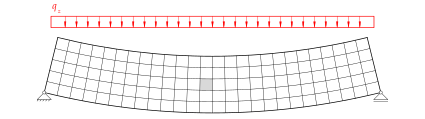
\includegraphics{index_files/mediabag/../images/Kontinua_system.pdf}

}

\caption{\label{fig-reine_biegung_system}Statisches System mit einer
Einteilung in differentielle Elemente}

\end{figure}

Die Abbildung~\ref{fig-system_reine_biegung_element} zeigt ein
herausgeschnittenes Element mit infinit kleinen Abmessungen. An den
Schnittkanten sind Schnittkräfte eingeführt. Ebenfalls ist der verformte
Zustand unterhalb dargestellt. Die Darstellung im verformten Zustand
liefert Auskunft über die kinematischen Relationen. Es wird angenommen,
dass das Element seiner Form treu bleibt, bzw. sich als ganzes verdreht.

\begin{figure}[H]

{\centering 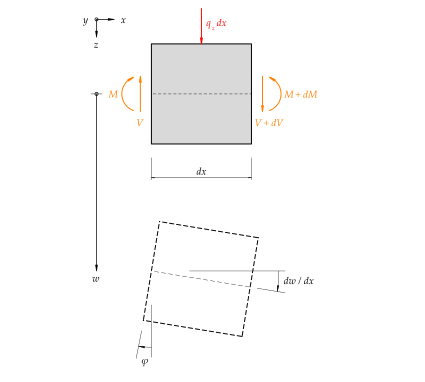
\includegraphics{index_files/mediabag/../images/Kontinua_element.pdf}

}

\caption{\label{fig-system_reine_biegung_element}Differentielles Element
des reinen Biegebalkens}

\end{figure}

Um die Beziehung des reinen Biegeträgers herzuleiten, sind neben den
Gleichgewichtsbedingungen und kinematischen Relationen ebenfalls die
Werkstoffbeziehungen erforderlich. Dies wird folgend bei der Herleitung
aufgegriffen.

\hypertarget{herleitung}{%
\subsection{Herleitung}\label{herleitung}}

Beginnend bei den Gleichgewichtsbetrachtungen kann anhand des
Gleichgewichts der vertikalen Kräfte die Gleichung~\ref{eq-dgl_v_x}
emittelt werden. Diese beschreibt die Beziehung zwischen Einwirkung und
Querkraft.

\[
\downarrow^+\sum F_z = 0 = q_z(x)\cdot dx -V + (V+dV)
\]

\[
q_z(x)\cdot dx = - dV
\]

\begin{equation}\protect\hypertarget{eq-dgl_v_x}{}{
q_z(x) = \frac{dV}{dx} = -V(x)'     
}\label{eq-dgl_v_x}\end{equation}

Aus dem Gleichgewicht der Momente folgt die Gleichung~\ref{eq-dgl_M_y},
welche die Beziehung zwischen Einwirkung und Biegemoment darstellt.

\[
\sum^{\curvearrowleft+} M_y = 0 = (M+dM) - M - V \cdot dx + q_z(x)\cdot dx \cdot dx/2
\]

Dabei kann der Anteil aus der Einwirkung \(q_z(x)\cdot dx \cdot dx/2\)
vernachlässigt werden, da dieser von höherer Ordnung klein ist. Es
folgt:

\[
0 = dM - V \cdot dx
\]

Wird diese Beziehung umgeformt, so resultiert die Beziehung zwischen
Querkraft und Biegemoment: \[
V = \frac{dM}{dx} 
\]

Abschliessend lässt sich unter Berücksichtigung der
Gleichung~\ref{eq-dgl_v_x} die Gleichung~\ref{eq-dgl_M_y} definieren:
\begin{equation}\protect\hypertarget{eq-dgl_M_y}{}{
q_z(x) = -V(x)'= -M(x)''
}\label{eq-dgl_M_y}\end{equation}

Mittels Gleichgewicht lassen sich keine weiteren Beziehungen ermitteln.
Berücksichtigt man die Werkstoffbeziehungen und kinematischen
Relationen, so lassen sich Aussagen zwischen Einwirkung und Verformung
definieren. Um die Herleitung abzukürzen wird die Beziehung in
Gleichung~\ref{eq-momentenkrümmung} zwischen Biegemoment und Krümmung
vorausgesetzt.

\begin{equation}\protect\hypertarget{eq-momentenkruxfcmmung}{}{
\frac{M}{EI} = \chi
}\label{eq-momentenkrümmung}\end{equation}

Allgemein gilt, die Krümmung entspricht der Änderung der Verdrehung:

\begin{equation}\protect\hypertarget{eq-krummung}{}{
\chi = \varphi(x)'
}\label{eq-krummung}\end{equation}

Aus der verformten Lage in
Abbildung~\ref{fig-system_reine_biegung_element} lässt sich die
Verdrehung des Elements bestimmen. Da das Element seiner Form treu
bleibt, entspricht die Verdrehung der Änderung der Verformung.

\[
-\varphi = \frac{dw}{dx}
\]

Daraus folgt die Beziehung zwischen Biegemoment und Verformung:

\[
M = -EIw(x)''
\]

und unter Berücksichtigung der Gleichung~\ref{eq-dgl_M_y} folgt die
Beziehung zwischen Verformung und Einwirkung, dargestellt in
Gleichung~\ref{eq-dgl_reine_biegung}.
\begin{equation}\protect\hypertarget{eq-dgl_reine_biegung}{}{
q(x) = EIw(x)''''
}\label{eq-dgl_reine_biegung}\end{equation}

Durch das Lösen der Differentialgleichung lassen sich die Zustandslinien
der Querkräfte, Biegemomente, Verdrehungen und Verformungen bestimmen.

\hypertarget{grenzen-der-anwendung}{%
\subsection{Grenzen der Anwendung}\label{grenzen-der-anwendung}}

Das Modell berücksichtigt keine Schubverformungen. Da in der Praxis
übliche Stahlbetonbauteile eine signifikant grössere Schubsteifigkeit
als Biegesteifigkeit aufweisen, liefert das Modell zuverlässige
Resultate. Sowie gilt, die Gleichung~\ref{eq-dgl_reine_biegung} lässt
lediglich die Anwendung einer konstanten Biegesteifigkeit zu.

\hypertarget{sec-mohrsche_analogie}{%
\section{Mohr'sche Analogie}\label{sec-mohrsche_analogie}}

Die Mohr'sche Analogie ist an sich keine Modellvorstellung, sondern
beschreibt ein handhabbares Lösungsvorgehen der Differentialgleichung
für reine Biegeträger.

\hypertarget{aufbau-1}{%
\subsection{Aufbau}\label{aufbau-1}}

Aus den Beziehungen, detailliert beschrieben in
Kapitel~\ref{sec-kontinua}, können folgende Abhängigkeiten definiert
werden:

\begin{equation}\protect\hypertarget{eq-mohr1}{}{
\frac{d^2M}{dx^2} = M'' = -q_z
}\label{eq-mohr1}\end{equation}

\begin{equation}\protect\hypertarget{eq-mohr2}{}{
\frac{d^2w}{dx^2} = w'' = -\frac{M}{EI}
}\label{eq-mohr2}\end{equation}

Erkennbar ist die Analogie der beiden Gleichungen. Aus der Einwirkung
lässt sich der Verlauf der Biegemomente bestimmen. Wird nun auf ein
analoges System der Verlauf der Biegemomente dividiert durch die
Biegesteifigkeit als Einwirkung angesetzt, so lässt sich mit dem
gleichen Berechnungsvorgehen die Verformung bestimmen. Lediglich den
Randbedingungen ist Beachtung zu schenken, welche mit entsprechenden
Lagerungsbedingungen im analogen System berücksichtigt werden. Die
Anpassung der Lagerungsbedingungen für ein analoges System ist in
Abbildung~\ref{fig-randbedingungen_analogiesysteme} gezeigt.

\begin{figure}[H]

{\centering 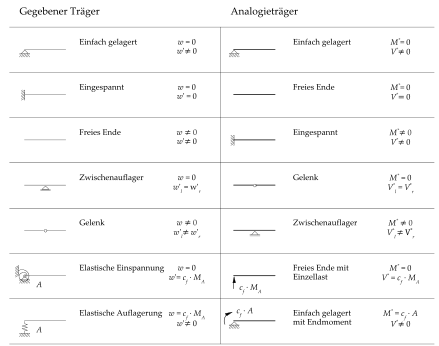
\includegraphics{index_files/mediabag/../images/analogietrager.pdf}

}

\caption{\label{fig-randbedingungen_analogiesysteme}Lagerungsbedingungen
für Analogiesysteme, übernommen aus
{[}\protect\hyperlink{ref-Spathelf2022}{4}{]}}

\end{figure}

Die Mohr'sche Analogie ermöglicht folglich die Bestimmung der
Verformungen durch das Ermitteln zweier Biegemomentenverläufe, am realen
und am analogen System.

\hypertarget{sec-norm}{%
\section{Abschätzung nach Norm}\label{sec-norm}}

Die folgende Beschreibung richtet sich nach der Masterthesis
{[}\protect\hyperlink{ref-Stecher2022}{5}{]}. Sowie sind die Beziehungen
empirischen Ursprungs.

Der Schweizerische Ingenieuren- und Architekten Verband (SIA) stellt in
ihrer aktuellen Betonnorm {[}\protect\hyperlink{ref-SIA2013a}{6}{]}
Ziffer 4.4.3.2.5 den Ansatz in Gleichung~\ref{eq-w_1_II_sia} zur
Ermittlung der Verformung im gerissenen Zustand. Dazu ist die elastische
ungerissene Verformung zu bestimmen und mit einem Faktor, welcher
abhängig von Zug- und Druckbewehrungsgehalt, der Kriechzahl sowie der
Geometrie ist, zu vergrössern. Das Verhalten des Faktors unter
Variierung der Bewehrungsgehälter mit konstanter Höhe und konstanter
statischer Höhe ist in Abbildung~\ref{fig-fg} gezeigt.

\begin{equation}\protect\hypertarget{eq-w_1_II_sia_faktor}{}{
w_{1II,SIA} = f_g w_1
}\label{eq-w_1_II_sia_faktor}\end{equation}

\begin{equation}\protect\hypertarget{eq-w_1_II_sia}{}{
w_{1II,SIA} = \frac{1-20\rho'}{10\rho^{0.7}}(0.75+0.1\varphi)\left(\frac{h}{d}\right)^3 w_1
}\label{eq-w_1_II_sia}\end{equation}

Durch die Vernachlässigung der Druckbewehrung, sowie ohne
Berücksichtigung von Langzeiteinflüssen, sprich das Kriechen, folgt die
Gleichung~\ref{eq-w_1_II_sia_simple}.

\begin{equation}\protect\hypertarget{eq-w_1_II_sia_simple}{}{
w_{1II,SIA} = \frac{0.75}{10\rho^{0.7}}\left(\frac{h}{d}\right)^3 w_1
}\label{eq-w_1_II_sia_simple}\end{equation}

\begin{figure}[H]

{\centering 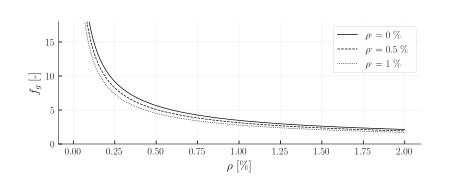
\includegraphics{index_files/mediabag/../images/f_g.pdf}

}

\caption{\label{fig-fg}Verlauf des Vergrösserungsfaktors der Abschätzung
nach Norm}

\end{figure}

\hypertarget{sec-zuggurtmodell}{%
\section{Zuggurtmodell}\label{sec-zuggurtmodell}}

Das Zuggurtmodell beschreibt das Verformungsverhalten nach dem Reissen
des Betons. Das Modell findet Anwendung bei der Ermittlung der
gerissenen Biegesteifigkeit.

\hypertarget{aufbau-2}{%
\subsection{Aufbau}\label{aufbau-2}}

Der folgende Abschnitt beschreibt das Zuggurtmodell anhand der
Herleitungen in {[}\protect\hyperlink{ref-Spathelf2022}{4}{]}. Das
Zuggurtmodell betrachtet auf Zug beanspruchte Stahlbetonzugglieder. Das
Modell erlaubt eine Eingrenzung der Rissbreiten und der Rissabstände. Im
Bereich zwischen den Rissen erhöht sich die Steifigkeit des Zugglieds,
da sich der Beton am Lastabtrag beteiligt. Dies wird als Zugversteifung
beschrieben. Um das Verhalten des Verbunds zwischen Beton und Betonstahl
im ungerissenen Bereich zu definieren, wird eine
Verbundschubspannungs-Schlupf-Beziehung dem Modell zugrunde gelegt.

\begin{figure}[H]

{\centering 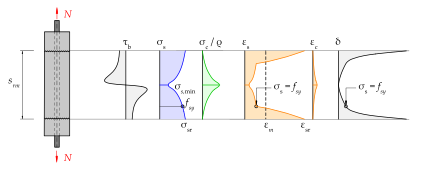
\includegraphics{index_files/mediabag/../images/Zuggurtmodell_grund.pdf}

}

\caption{\label{fig-zuggurtmodell}Verlauf der effektiven
Verbundschubspannungen, Betonstahlspannungen, Betonspannungen,
Betonstahldehnungen, Betondehnungen und Schlupf bei einem Zugglied. Bild
neu gezeichnet nach {[}\protect\hyperlink{ref-Spathelf2022}{4}{]}}

\end{figure}

Verwendet wird eine abegtreppte, starr-ideal-plastische
Verbundschubspannungs-Schlupf-Beziehung. Durch die Idealisierung lassen
sich die Spannungen und Dehnungen ausschliesslich durch
Gleichgewichtsbeziehungen ermitteln. Die Abtreppung erfolgt beim
Erreichen der Fliessgrenze des Betonstahls. In der
Abbildung~\ref{fig-zuggurtmodell} im Verlauf des Schlupfs (rechts) ist
die Position der Fliessspannung dargestellt.

\begin{figure}[H]

{\centering 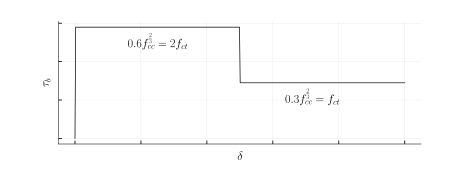
\includegraphics{index_files/mediabag/../images/verbund_schlupf.pdf}

}

\caption{\label{fig-verbund_schlupf}Idealisierte
Verbundschubspannungs-Schlupf-Beziehung}

\end{figure}

Zudem verdeutlicht der Verbunschubspannungsverlauf, in
Abbildung~\ref{fig-zuggurtmodell} (links), die Rechtfertigung der
Vereinfachung als abgetreppten Verlauf.

\hypertarget{ansatz-nach-marti}{%
\subsubsection{Ansatz nach Marti}\label{ansatz-nach-marti}}

In {[}\protect\hyperlink{ref-Spathelf2022}{4}{]} wird der Ansatz von
Marti zur Berücksichtigung der Zugversteifung basierend auf dem
Zuggurtmodell für Biegeelemente aufgezeigt.

Vor dem Erreichen der Zugfestigkeit des Betons verbleibt das Zugglied
ungerissen und verhält sich linear elastisch. Beim Reissen des
Querschnitts verharrt die Betonspannung bei der Rissspannung. Eine
Erhöhung der Einwirkung erhöht lediglich die Zugspannung im Betonstahl.

\begin{figure}[H]

{\centering 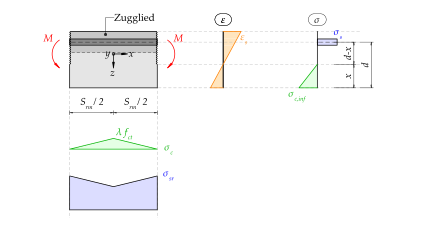
\includegraphics{index_files/mediabag/../images/QS_zugversteifung.pdf}

}

\caption{\label{fig-einfluss_zugversteifung}Einfluss der
zugversteifenden Wirkung bei einem Biegeelement}

\end{figure}

In der Abbildung~\ref{fig-einfluss_zugversteifung} ist der
Spannungsverlauf des Betons und des Betonstahls gezeigt. Diese zeigt die
Abnahme der Betonstahlspannung bei steigender Entfernung zum Riss. Mit
der Spannungsreduktion folgt eine Dehnungsreduktion, welche mit
\(\Delta \varepsilon_s (\lambda)\) beschrieben wird. Aus der
Dehnungsreduktion lässt sich eine Krümmungsdifferenz definieren nach
Gleichung~\ref{eq-krummungsdiff}.

\begin{equation}\protect\hypertarget{eq-krummungsdiff}{}{
\Delta \chi(\lambda) = \frac{\Delta \varepsilon_s (\lambda)}{(d-x)} = \frac{\lambda}{2} \cdot \left ( \frac{M_r}{EI^{II}} - \frac{f_{ct}}{E_c\cdot(d-x)}\right )
}\label{eq-krummungsdiff}\end{equation}

Dabei wird die gesamte Krümmung \(M_r/EI^{II}\) beim Reissen des
Querschnitts durch die Krümmung beim Erreichen der Zugfestigkeit des
Betons \(f_{ct}/(E_c\cdot(d-x))\) reduziert. Die
Gleichung~\ref{eq-krummungsdiff} kann mittels dem effektiven
Bewehrungsgehalt formuliert werden.

\begin{equation}\protect\hypertarget{eq-rho_eff}{}{
\rho_{\text{eff}} = \left [\frac{M_r(d-x)\cdot E_S}{f_{ct}\cdot EI^{II}}+1-n \right ]^{-1}
}\label{eq-rho_eff}\end{equation}

\begin{equation}\protect\hypertarget{eq-krummungsdiff_2}{}{
\Delta \chi(\lambda) = \frac{\lambda}{2} \cdot \frac{f_{ct} \cdot (1-\rho_{\text{eff}})}{\rho_{\text{eff}} \cdot E_s \cdot (d-x)}
}\label{eq-krummungsdiff_2}\end{equation}

Das Modell liefert ebenfalls Beziehungen zur Bestimmung der Rissweite
und der Rissabstände.
\begin{equation}\protect\hypertarget{eq-rissabstand_marti}{}{
s_{rm} = \frac{\oslash_{s} \lambda \left(1 - \rho_{\text{eff}}\right)}{4 \rho_{\text{eff}}}
}\label{eq-rissabstand_marti}\end{equation}

\begin{equation}\protect\hypertarget{eq-rissweite_marti}{}{
w_{r} = \frac{s_{rm} \left(- \lambda \sigma_{sr0} + 2 \sigma_{sr}\right)}{2 E_{s}}
}\label{eq-rissweite_marti}\end{equation}

Der Modellbeschrieb wird mit der Erläuterung des \(\lambda\)-Beiwerts
abgeschlossen. Grundsätzlich gilt die Annahme, dass sich ein Riss
einstellt beim Erreichen der Zugfestigkeit des Betons.

\begin{figure}[H]

{\centering 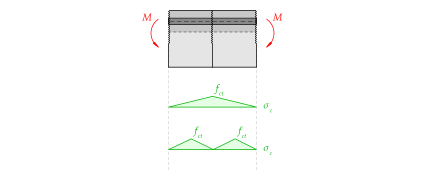
\includegraphics{index_files/mediabag/../images/lambda_beiwert.pdf}

}

\caption{\label{fig-fallunterscheidung_lambda_riss}Fallunterscheidung
beim Erreichen der Zugfestigkeit des Betons}

\end{figure}

Vor dem Erreichen der Zugfestigkeit des Betons reisst der Beton nicht.
Unmittelbar beim Erreichen der Zugfestigkeit stellt sich der Riss ein.
Betrachtet man die Abbildung~\ref{fig-fallunterscheidung_lambda_riss},
kann in der Elementmitte die Zugfestigkeit erreicht werden, oder sich
ein erneuter Riss bilden. Der Beiwert \(\lambda\) dient folglich zur
Unterscheidung dieser Grenzwerte.

\hypertarget{grenzen-der-anwendung-1}{%
\subsubsection{Grenzen der Anwendung}\label{grenzen-der-anwendung-1}}

Das Zuggurtmodell findet Anwendung bei Zuggliedern in der Biegezugzone.
Es liefert Auskunft über Rissweiten und Rissbreiten, sowie eine
Verfeinerung der Biegesteifigkeit im gerissenen Bereich. Das Modell
beschränkt sich ausschliesslich auf normalzugbeanspruchte Bauteile.

\hypertarget{sec-numint}{%
\section{Numerische Integration der Krümmung}\label{sec-numint}}

Die numerische Integration der Krümmung bietet einen Ansatz, einen
nicht-linearen Biegesteifigkeitenverlauf zu berücksichtigen. Mittels der
Arbeitsgleichung lassen sich die Verformungen punktuell bestimmen. Für
Biegeträger gilt die folgende Gleichung~\ref{eq-arbeitsgleichung}.

\begin{equation}\protect\hypertarget{eq-arbeitsgleichung}{}{
w = \int_0^l \bar{M}(x) \cdot \frac{M(x)}{EI} d_x
}\label{eq-arbeitsgleichung}\end{equation}

Wobei \(\frac{M(x)}{EI} = \chi(x)\) gilt, sprich dem Krümmungsverlauf
entspricht. Die Arbeitsgleichung setzt die innere Arbeit aus dem
Biegemoment multipliziert mit der Krümmung zu der äusseren Arbeit
gleich, welche aus Kraft multipliziert mit dem Weg entspricht. Daraus
lässt sich der Weg, sprich die Verformung herauslösen.

\hypertarget{momenten-kruxfcmmungs-beziehung}{%
\subsection{Momenten-Krümmungs-Beziehung}\label{momenten-kruxfcmmungs-beziehung}}

Eine nicht-lineare Momenten-Krümmungs-Beziehung lässt sich händisch
mittels einer Querschnittsanalyse bestimmen. Zur rechnerischen
Ermittlung gelten folgende Annahmen, wie in
{[}\protect\hyperlink{ref-Spathelf2022}{4}{]} beschrieben:

\begin{itemize}
\tightlist
\item
  Eben- und senkrechtbleiben der Querschnitte
\item
  Die Betonzugfestigkeit \(f_{ct}\) wird für Zustände nach dem
  Überschreiten von \(f_{ct}\) vernachlässigt
\item
  Die Bewehrung überträgt Zug- und Druckkräfte ausschliesslich in
  Stabrichtung
\end{itemize}

Dazu wird der Querschnitt bei steigender Dehnung, induziert durch
Biegung, analysiert. Der entsprechende Biegewiderstand und die
gekoppelte Krümmung wird dabei bestimmt. Grundsätzlich wird der
Querschnitt vor dem Reissen des Betons, nach dem Reissen, beim
Fliessbeginn der Zugbewehrung und beim Erreichen des Biegewiderstands
betrachtet. Exemplarisch ist in Abbildung~\ref{fig-exemplar_qs_analyse}
der Zustand des Biegewiderstands dargestellt.

\begin{figure}[H]

{\centering \includegraphics{index_files/mediabag/../images/QS_14_analyse_1.pdf}

}

\caption{\label{fig-exemplar_qs_analyse}Querschnittsanalyse für den
Zustand des Biegewiderstands}

\end{figure}

\hypertarget{sec-fachwerk}{%
\section{Fachwerksanalyse}\label{sec-fachwerk}}

Die Fachwerksanalyse basiert auf einer Modellierung mittels
Spannungsfeldern. Das Ziel ist es, mittels Spannungsfelder den
Kraftfluss im Balken nachzuverfolgen. Das Fachwerk bildet den Kraftfluss
detaillierter als eine Querschnittsanalyse ab. In Anlehnung an die
Modellierungsstufen in {[}\protect\hyperlink{ref-Thoma2020}{7}{]}
gliedert sich die Fachwerksmodellierung im level of Approximation II an,
eine Stufe höher als die Querschnittsanalyse. Grundsätzlich wird das
Modell jedoch zur Bemessung im Grenzzustand der Tragsicherheit
verwendet. Folgend wird beschrieben, wie mittels diesem Deformationen
zielführend bestimmt werden können.

\hypertarget{spannungsfelder}{%
\subsection{Spannungsfelder}\label{spannungsfelder}}

Der Kraftfluss lässt sich für die in dieser Arbeit untersuchten Versuche
mit nicht-zentrierten Fächern und Parallelfeldern modellieren. Durch die
Wahl eines Neigungswinkels der Felder ergibt sich deren Breite. Bei der
Bemessung im Grenzzustand der Tragsicherheit ist die Neigung der
Druckfelder frei wählbar. Durch die Variation des Winkels ändert sich
die Kraftaufteilung zwischen der Schubbewehrung und der Zugbewehrung.

\hypertarget{wahl-des-neigungswinkels}{%
\subsubsection{Wahl des
Neigungswinkels}\label{wahl-des-neigungswinkels}}

Anders als beim Entwurf der Balken, ist die Wahl der Bügelbewehrung bei
der Nachrechnung bereits festgelgt. Folgend wird eine Abschätzung zur
Wahl des Neigungswinkels aufgezeigt. Die Querkraftbemessung der
Betonnorm {[}\protect\hyperlink{ref-SIA2013a}{6}{]} basiert auf der
Modellierung mittels Spannungsfeldern. Der Neigungswinkel der
Betondruckstrebe kann in Anlehnung an die
Gleichung~\ref{eq-v_rds_sia262} zur Bestimmung des Querkraftwiderstands
von vertikaler Schubbewehrung, gemäss Ziffer 4.3.3.4.3, bestimmt werden.

\begin{equation}\protect\hypertarget{eq-v_rds_sia262}{}{
V_{Rd,s} = \frac{A_{sw}}{s} z f_{sd} \cot(\alpha)
}\label{eq-v_rds_sia262}\end{equation}

Wird nun ein Fachwerkmodell für die Nachrechnung von Verformungen von
Versuchen verwendet, so gilt es den passenden Neigungswinkel anhand der
gegebenen Schubbewehrung zu ermitteln. Dabei wird vom Bruchzustand
ausgegangen. Somit wird die maximale Querkraft, der Hebelarm der inneren
Kräfte des Biegewiderstands, die Fliess- oder Bruchspannung der
Bügelbewehrung und die entsprechende Querschnittsfläche in die
Gleichung~\ref{eq-v_rds_sia262} eingesetzt. Daraus lässt sich die
Neigung bestimmen. Mit dem bestimmten Neigungswinkel ist die Geometrie
der Spannungsfelder und folglich die des Fachwerks eindeutig bestimmt.

\hypertarget{dehnsteifigkeiten}{%
\subsubsection{Dehnsteifigkeiten}\label{dehnsteifigkeiten}}

Abschliessend gilt es den Pendelstäben die entsprechenden
Querschnittsflächen, bzw. Dehnsteifigkeiten zuzuordnen, um die passenden
Verformungen zu berechnen. In den Versuchsnachrechnungen des Dreipunkt-
und Vierpunktbiegeversuchs ist dies detailliert aufgezeigt.

\hypertarget{sec-versatzmass}{%
\section{Versatzmass}\label{sec-versatzmass}}

Abgeschlossen wird die Modellbeschreibung mit der Beschreibung des
Versatzmasses. Die Modellierung mittels Spannungsfeldern zeigt, dass die
Querkraft durch ein diagonales Druckfeld abgetragen wird. Die
horizontale Komponente des diagonalen Kraftvektors erhöht die
Längskraft. Eine Erhöhung der Längskraft bringt eine Erhöhung des
Biegemoments mit sich.

\begin{figure}[H]

{\centering 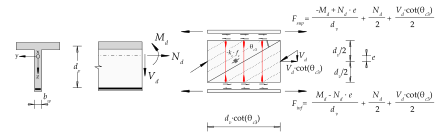
\includegraphics{index_files/mediabag/../images/spannungsfeld_versatzmass.pdf}

}

\caption{\label{fig-laengszug_spf}Längszugkraft aus der Querkraft,
dargestellt im Spannungsfeld, entnommen aus
{[}\protect\hyperlink{ref-Thoma2020}{7}{]}}

\end{figure}

Visualisiert ist dies in der Abbildung~\ref{fig-laengszug_spf}. Es ist
ein freigeschnittenes Spannungsfeld gezeigt, welches mit Schnittkräften
ergänzt ist, um das Gleichgewicht im System zu wahren. Die diagonal
gerichtete Druckkraft, mit deren horizontalen Komponente ist am
Schnittufer gezeigt. Durch das Anwenden des Gleichgewichts lassen sich
die Gurtkräfte bestimmen, welche durchwegs durch den Term in der
Gleichung~\ref{eq-versatzmass} erhöht werden.

\begin{equation}\protect\hypertarget{eq-versatzmass}{}{
h_{versatz} = \frac{V \cdot \cot(\theta_{c3})}{2}
}\label{eq-versatzmass}\end{equation}

\begin{equation}\protect\hypertarget{eq-versatzmoment}{}{
M_{versatz} = \frac{V \cdot \cot(\theta_{c3})}{2} \cdot z
}\label{eq-versatzmoment}\end{equation}

Die Gleichung~\ref{eq-versatzmass} beschreibt die Erhöhung der
Längszugkraft aus der Querkraft. Der Einfluss auf das Biegemoment aus
der erhöhten Längszugkraft zeigt die Gleichung~\ref{eq-versatzmoment}.

\bookmarksetup{startatroot}

\hypertarget{sec-dreipunkt}{%
\chapter{Dreipunktbiegeversuch}\label{sec-dreipunkt}}

In diesem Kapitel werden alle in Kapitel~\ref{sec-modellbeschrieb}
beschriebenen Modelle auf einen Dreipunktbiegeversuch angewendet. Das
primäre Ziel ist es, die Differenzen zwischen den mit den verschiedenen
Modellen berechneten Verformungen und den tatsächlich gemessenen
Verformungen aufzuzeigen. Der Schwerpunkt liegt auf der Anwendung der
Modelle. Das Kapitel endet mit einem Vergleich der verschiedenen Modelle
und einer Diskussion der Ergebnisse.

\hypertarget{versuchsbeschreibung}{%
\section{Versuchsbeschreibung}\label{versuchsbeschreibung}}

Der Versuch A3 in der zweiten Versuchsanordnung (kurz A3V2) aus
{[}\protect\hyperlink{ref-Jaeger2006}{1}{]} dient als Grundlage. Der
Körper wurde in der ersten Versuchsanordnung bereits belastet, jedoch
unterschiedlich gelagert. Trotzdem führt dies zu Vorverformungen in der
zweiten Versuchsanordnung. Im Folgenden sind die wesentlichen Eckdaten
des Versuchs dargestellt, während detaillierte Beschreibungen in
{[}\protect\hyperlink{ref-Jaeger2006}{1}{]} zu finden sind. Der Versuch
beinhaltet einen Plattenstreifen, dessen Lagerung einem
Dreipunktbiegeversuch entspricht. Der Plattenstreifen wird durch \(F_A\)
bis zum Bruch belastet. Die maximale Last beträgt \(331 \text{ kN}\).

\begin{figure}[H]

{\centering 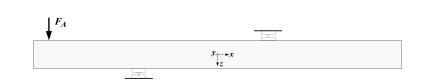
\includegraphics{index_files/mediabag/../images/belastung_a3v2.pdf}

}

\caption{Lagerung und Belastung des Plattenstreifens, entnommen aus
{[}\protect\hyperlink{ref-Jaeger2006}{1}{]}}

\end{figure}

Das Bewehrungslayout ist so konzipiert, dass nur eine Zugbewehrung im
Bereich der negativen Momente vorhanden ist. Die Bewehrung ist
orthogonal bzw. parallel zu den Bauteilkanten verlegt. Dargestellt ist
die Bewehrungsführung in der Abbildung~\ref{fig-bewehrung_a3v2}.

\begin{figure}[H]

{\centering \includegraphics{index_files/mediabag/../images/bewehrung_a3v2.pdf}

}

\caption{\label{fig-bewehrung_a3v2}Bewehrungslayout des
Plattenstreifens, entnommen aus
{[}\protect\hyperlink{ref-Jaeger2006}{1}{]}}

\end{figure}

Die vorhandene Querkraftbewehrung, ausgeführt als Schubdübel, ermöglicht
ein weitgehend durch Biegung verursachtes Versagen. Dies entspricht der
Abgrenzung, primär Biegeverformungen zu betrachten. Das
Last-Verformungs-Verhalten an der Stelle \(w_1\) ist in der
Abbildung~\ref{fig-lastverformung_a3v2} dargestellt. Es zeigt sich ein
deutlicher Bereich des Fliessens der Zugbewehrung ohne vorzeitiges
Querkraftversagen. Erkennbar ist dies an der Erhöhung der Verformung
ohne markante Steigerung der Last. Aufgezeigt ist ebenfalls die
Vorverformung aus der ersten Versuchsanordnung.

\begin{figure}[H]

{\centering 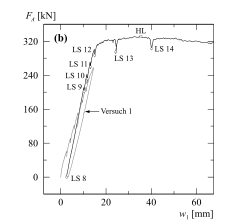
\includegraphics[width=\textwidth,height=90mm]{index_files/mediabag/../images/eth-28720-01_versuche_jaeger103.pdf}

}

\caption{\label{fig-lastverformung_a3v2}Last-Verformungs-Verhalten des
Plattenstreifens, entnommen aus
{[}\protect\hyperlink{ref-Jaeger2006}{1}{]}}

\end{figure}

In Abbildung~\ref{fig-verformungsverlauf_a3v2} ist der
Verformungsverlauf entlang der Stabachse dargestellt. Der Verlauf zeigt,
dass die maximalen Verformungen bei der Krafteinleitung entstehen.

\begin{figure}[H]

{\centering 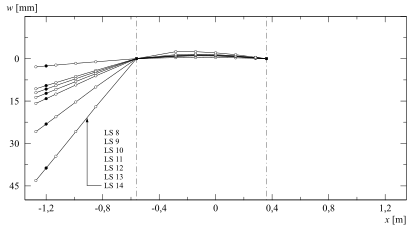
\includegraphics{index_files/mediabag/../images/eth-28720-01_versuche_jaeger104.pdf}

}

\caption{\label{fig-verformungsverlauf_a3v2}Verformungsverlauf des
Plattenstreifens, entnommen aus
{[}\protect\hyperlink{ref-Jaeger2006}{1}{]}}

\end{figure}

\hypertarget{eigenschaften-der-baustoffe}{%
\section{Eigenschaften der
Baustoffe}\label{eigenschaften-der-baustoffe}}

Die Betoneigenschaften wurden in
{[}\protect\hyperlink{ref-Jaeger2006}{1}{]} mittels Würfel- und
Zylinderproben ermittelt. Ebenso wurden die Eigenschaften des
Betonstahls durch Zugproben bestimmt. Um von den Druckfestigkeiten der
Zylinderproben auf die Bauteildruckfestigkeit zu schliessen, sind in
{[}\protect\hyperlink{ref-Jaeger2014}{8}{]} Transformationsbeziehungen
beschrieben. Folgend ist die Anwendung dieser aufgezeigt. Die
Betondruckfestigkeit aufgrund der Zylinderdruckfestigkeit entspricht:

\begin{equation}f_{c} = 2.7 f_{cc}^{\frac{2}{3}}\end{equation}

\begin{equation}f_{c} = \frac{40.827 \text{N}}{\text{mm}^{2}}\end{equation}

Ebenfalls kann die Zugfestigkeit gemäss
{[}\protect\hyperlink{ref-Jaeger2013}{9}{]} anhand der
Zylinderdruckfestigkeit bestimmt werden.

\begin{equation}f_{ct} = 0.3 f_{cc}^{\frac{2}{3}}\end{equation}

\begin{equation}f_{ct} = \frac{4.54 \text{N}}{\text{mm}^{2}}\end{equation}

Abschliessend wir der Elastizitätsmodul nach
{[}\protect\hyperlink{ref-Jaeger2013}{9}{]} abgeschätzt.

\begin{equation}E_{c} = 10000 \sqrt[3]{f_{cc}}\end{equation}

\begin{equation}E_{c} = \frac{38886.0 \text{N}}{\text{mm}^{2}}\end{equation}

\hypertarget{reiner-biegetruxe4ger}{%
\section{Reiner Biegeträger}\label{reiner-biegetruxe4ger}}

In diesem Abschnitt wird das in Kapitel~\ref{sec-kontinua} beschriebene
Modell auf das Versuchsobjekt angewendet. Zunächst wird das statische
System des Versuchs in Abbildung~\ref{fig-system_2} dargestellt.

\begin{figure}[H]

{\centering \includegraphics{index_files/mediabag/../images/System_anordnung_2.pdf}

}

\caption{\label{fig-system_2}Statisches System des Plattenstreifens}

\end{figure}

Eine Vereinfachung des in Abbildung~\ref{fig-system_2} dargestellten
Systems ist in Abbildung~\ref{fig-system_2_lager} zu sehen. Dabei wird
das Eigengewicht aufgrund seines minimalen Einflusses auf das
Biegemoment vernachlässigt. Darüber hinaus wurden die Verformungen, die
in {[}\protect\hyperlink{ref-Jaeger2006}{1}{]} gemessen wurden, nach der
Installation des Trägers erfasst. Daher spiegelt die Messung den
Einfluss des Eigengewichts nicht wider.

\begin{equation}\protect\hypertarget{eq-eigengewicht}{}{
g_M, g_{k1}, g_{k2} = 0
}\label{eq-eigengewicht}\end{equation}

Die Berücksichtigung der Lagerbreiten führt zur Streckenlast \(f_A\),
bzw. zu den Lagerreaktionen \(f_B\) und \(f_C\). Aufgezeigt ist dies in
der Abbildung~\ref{fig-system_2_lager}.

\begin{figure}[H]

{\centering \includegraphics{index_files/mediabag/../images/System_anordnung_2_lagerbreite.pdf}

}

\caption{\label{fig-system_2_lager}Angepasstes statisches System des
Plattenstreifens}

\end{figure}

Die nun folgenden Berechnungen beziehen sich ausschliesslich auf das
System in der Abbildung~\ref{fig-system_2_lager}. Dabei werden die
Parameter in der Tabelle~\ref{tbl-params_reiner_biegetraeger}
berücksichtigt.

\hypertarget{tbl-params_reiner_biegetraeger}{}
\begin{longtable}[]{@{}
  >{\raggedright\arraybackslash}p{(\columnwidth - 2\tabcolsep) * \real{0.5000}}
  >{\raggedright\arraybackslash}p{(\columnwidth - 2\tabcolsep) * \real{0.5000}}@{}}
\caption{\label{tbl-params_reiner_biegetraeger}Berechnungsparameter der
Systemgeometrie}\tabularnewline
\toprule\noalign{}
\begin{minipage}[b]{\linewidth}\raggedright
Parameter
\end{minipage} & \begin{minipage}[b]{\linewidth}\raggedright
\hspace{0pt}
\end{minipage} \\
\midrule\noalign{}
\endfirsthead
\toprule\noalign{}
\begin{minipage}[b]{\linewidth}\raggedright
Parameter
\end{minipage} & \begin{minipage}[b]{\linewidth}\raggedright
\hspace{0pt}
\end{minipage} \\
\midrule\noalign{}
\endhead
\bottomrule\noalign{}
\endlastfoot
\(a_{1} = 0.11 \text{m}\) & \(a_{2} = 0.64 \text{m}\) \\
\(a_{3} = 0.92 \text{m}\) & \(a_{4} = 0.95 \text{m}\) \\
\(b = 800.0 \text{mm}\) & \(b_{Auflager} = 100 \text{mm}\) \\
\(h = 200.0 \text{mm}\) & \hspace{0pt} \\
\end{longtable}

\hypertarget{auflagerkruxe4fte}{%
\subsection{Auflagerkräfte}\label{auflagerkruxe4fte}}

Zunächst müssen die Einwirkungen auf den Stab bestimmt werden, dazu sind
die Auflagerreaktionen erforderlich. Das statisch bestimmte System kann
mithilfe der Gleichgewichtsbeziehungen gelöst werden. Im Folgenden wird
die Gesamtlänge des Stabs bestimmt, als Kontrollgrösse der gewählten
Abstände.

\begin{equation}l_{tot} = a_{1} + a_{2} + a_{3} + a_{4}\end{equation}

\begin{equation}l_{tot} = 2.62 \text{m}\end{equation}

Durch das Aufstellen von Momentengleichgewichten um die Auflagerpunkte
\(C\) und \(B\) können die Beziehungen zwischen den Einwirkungen und den
Reaktionskräften ermittelt werden.

\begin{equation}0 = F_{A} a_{2} - F_{B} a_{3}\end{equation}

\begin{equation}0 = F_{A} \left(a_{2} + a_{3}\right) - F_{C} a_{3}\end{equation}

Durch das Auflösen der bestimmten Beziehungen folgen die
Auflagerreaktionen zu:

\begin{equation}F_{B} = \frac{F_{A} a_{2}}{a_{3}}\end{equation}

\begin{equation}F_{C} = \frac{F_{A} a_{2} + F_{A} a_{3}}{a_{3}}\end{equation}

Wie in Abbildung~\ref{fig-system_2_lager} gezeigt, gilt es die
Einzelkraft der Auflagerbreite entsprechend zu verteilen. Dies zeigen
die folgenden Gleichungen.

\begin{equation}f_{B} = \frac{F_{A} a_{2}}{a_{3} b_{Auflager}}\end{equation}

\begin{equation}f_{C} = \frac{F_{A} a_{2} + F_{A} a_{3}}{a_{3} b_{Auflager}}\end{equation}

\begin{equation}f_{A} = \frac{F_{A}}{b_{Auflager}}\end{equation}

\hypertarget{zustandslinien}{%
\subsection{Zustandslinien}\label{zustandslinien}}

Nach dem Bestimmen der Auflagerreaktionen können die Zustandslinien der
Schnittgrössen bestimmt werden. Die Zustandslinien der Schnittgrössen
resultieren aus der Bemühung der hergeleiteten Gleichungen in
Kapitel~\ref{sec-kontinua}. Dabei ist zu beachten, dass die
Zustandslinien lediglich für die maximal gewählte Laststufe dargestellt
sind. Der Verlauf der Einwirkungen ist in Abbildung~\ref{fig-q_x}
aufgezeigt.

\begin{figure}[H]

{\centering \includegraphics{index_files/mediabag/06_Versuch_2_A3_Jaeger_files/figure-pdf/fig-q_x-output-1.pdf}

}

\caption{\label{fig-q_x}Verlauf der Einwirkungen}

\end{figure}

Das Vorzeichen der Streckenlast gibt die Wirkungsrichtung an. Negative
Werte wirken entgegen der positiven \(z\)-Richtung. Die positive
\(z\)-Richtung ist in Abbildung~\ref{fig-system_2_lager} dargestellt.
Basierend auf dem Verlauf der Einwirkungen lässt sich der Verlauf der
Querkraft bestimmen. Durch Integration der Einwirkung über die
Laufvariable \(x\) ergibt sich der Verlauf, wie in
Gleichung~\ref{eq-vx_integriert} dargestellt.

\begin{equation}\protect\hypertarget{eq-vx_integriert}{}{
V(x) = -\int q(x) \, dx + c_1
}\label{eq-vx_integriert}\end{equation}

Mit der Randbedingung \(V(0) = 0\) kann die Integrationskonstante
bestimmt werden. Der Verlauf der Querkräfte ist in
Abbildung~\ref{fig-v_x} dargestellt. Die Querkräfte wirken in
\(z\)-Richtung.

\begin{figure}[H]

{\centering \includegraphics{index_files/mediabag/06_Versuch_2_A3_Jaeger_files/figure-pdf/fig-v_x-output-1.pdf}

}

\caption{\label{fig-v_x}Verlauf der Querkräfte}

\end{figure}

Nach dem bestimmten Querkraftverlauf folgt der Biegemomentenverlauf
unter der Bemühung der Gleichung~\ref{eq-m_x_a3v2}. Dazu ist der Verlauf
der Querkräfte zu integrieren.

\begin{equation}\protect\hypertarget{eq-m_x_a3v2}{}{
M(x) = \int V(x) \, dx + c_2
}\label{eq-m_x_a3v2}\end{equation}

Mit der Randbedingung \(M(0) = 0\) kann die Integrationskonstante
bestimmt werden. Der Verlauf der Biegemomente ist in
Abbildung~\ref{fig-m_x} dargestellt. Es ergibt sich ein Minimum über dem
Auflager \(C\).

\begin{figure}[H]

{\centering \includegraphics{index_files/mediabag/06_Versuch_2_A3_Jaeger_files/figure-pdf/fig-m_x-output-1.pdf}

}

\caption{\label{fig-m_x}Verlauf der Biegemomente}

\end{figure}

Zusätzlich zu den resultierenden Biegemomenten aus der Einwirkung kann
ein durch die Längszugkraft aus der Querkraft induziertes Biegemoment
ermittelt werden. Dies wird mit einem Versatzmass berücksichtigt.
Erläutert ist die Modellvorstellung in Kapitel~\ref{sec-versatzmass}.
Die Gleichung~\ref{eq-versatzmass} zeigt die Ermittlung des Versatzmass.
Multipliziert mit der statischen Höhe ergibt sich der Versatz des
Biegemoments aus Gleichung~\ref{eq-versatzmoment}. In der
Abbildung~\ref{fig-m_x_versatz} ist die Erhöhung durch das Versatzmass
gezeigt. Beim Momentenminimum bildet sich ein Plateau aus. Der
notwendige Hebelarm der inneren Kräfte ist anhand der statischen Höhe
\(d\) abgeschätzt. Die statische Höhe ist in
Abbildung~\ref{fig-qs_vereinfachung} dargestellt.

\begin{equation}d = - \frac{3 \oslash_{s}}{2} - c_{nom} + h\end{equation}

\begin{equation}d = 162.0 \text{mm}\end{equation}

Aus der berechneten statischen Höhe folgt der Hebelarm der inneren
Kräfte \(z\).

\begin{equation}z = 0.9 d\end{equation}

\begin{equation}z = 146.0 \text{mm}\end{equation}

Zur Bestimmung des Versatzmass gilt es die Neigung des Druckfelds zu
ermitteln. Abgeschätzt wird diese mit dem unteren Grenzwert des
definierten Bereichs aus der Norm
{[}\protect\hyperlink{ref-SIA2013a}{6}, p.~54{]}.

\begin{equation}\protect\hypertarget{eq-theta_c3}{}{
 \theta_{c3} = 30.0^{\circ} 
}\label{eq-theta_c3}\end{equation}

Unter diesen Annahmen folgt der Verlauf der Biegemomente mit dem
Versatzmass, dargestellt in der Abbildung~\ref{fig-m_x_versatz}.

\begin{figure}[H]

{\centering \includegraphics{index_files/mediabag/06_Versuch_2_A3_Jaeger_files/figure-pdf/fig-m_x_versatz-output-1.pdf}

}

\caption{\label{fig-m_x_versatz}Verlauf der Biegemomente, mit
Versatzmass}

\end{figure}

\hypertarget{verdrehung--und-verformungslinien}{%
\subsubsection{Verdrehung- und
Verformungslinien}\label{verdrehung--und-verformungslinien}}

Wie in Kapitel~\ref{sec-kontinua} hergeleitet, sind die
Gleichgewichtsbetrachtungen nicht ausreichend um die Verdrehung und
Verformung zu beschreiben. Die Werkstoffbeziehung bedingt eine
Biegesteifigkeit. Dabei wird von einer konstanten Biegesteifigkeit
ausgegangen. Unter der Annahme eines ungerissenen Betonquerschnitts
lässt sich die Biegesteifigkeit wie folgt berechnen:

\begin{equation}EI = \frac{E_{c} b h^{3}}{12}\end{equation}

\begin{equation}EI = 2.07 \cdot 10^{4} \text{kN} \text{m}^{2}\end{equation}

Der Verlauf der Verdrehung entspricht dem integrierten Verlauf der
Biegemomente, dividiert durch die Biegesteifigkeit.

\begin{equation}\protect\hypertarget{eq-verdrehung}{}{
\varphi(x) = \frac{1}{EI}\int M(x) \, dx + c_3
}\label{eq-verdrehung}\end{equation}

Die Verformung hingegen entspricht dem integrierten Verlauf der
Verdrehung.

\begin{equation}\protect\hypertarget{eq-verformung}{}{
w(x) = \int -\varphi(x) \, dx + c_4
}\label{eq-verformung}\end{equation}

Mit den Randbedingungen \(w(C) = 0\) und \(w(B) = 0\) können die
Integrationskonstanten bestimmt werden. Der elastische
Verformungsverlauf, bzw. der mit einer über die Stabachse konstanten
Biegesteifigkeit bestimmte Verformungsverlauf, ist in
Abbildung~\ref{fig-w_x} dargestellt.

\begin{figure}[H]

{\centering \includegraphics{index_files/mediabag/06_Versuch_2_A3_Jaeger_files/figure-pdf/fig-w_x-output-1.pdf}

}

\caption{\label{fig-w_x}Verlauf der Verformung, bestimmt mit einer
konstanten ungerissenen Biegesteifigkeit}

\end{figure}

\hypertarget{mohrsche-analogie}{%
\section{Mohr'sche Analogie}\label{mohrsche-analogie}}

In diesem Abschnitt sind die Zustandslinien der Schnittgrössen mittels
der Mohr'schen Analogie bestimmt. Das Vorgehen ist in
Kapitel~\ref{sec-mohrsche_analogie} beschrieben. Der bereits bestimmte
Momentenverlauf gemäss Abbildung~\ref{fig-m_x}, dividiert durch die
ungerissene Biegesteifigkeit, ist als Einwirkung auf das System
anzusetzen. Dies ist in Abbildung~\ref{fig-q_x_mohr} dargestellt.

\begin{figure}[H]

{\centering \includegraphics{index_files/mediabag/06_Versuch_2_A3_Jaeger_files/figure-pdf/fig-q_x_mohr-output-1.pdf}

}

\caption{\label{fig-q_x_mohr}Verlauf der Einwirkungen des
Analogiesystems}

\end{figure}

Die Randbedingungen bzw. die Lagerungen für das analoge System sind zu
ermitteln. Dies kann grundsätzlich mit den Lagerungsbedingungen aus
Abbildung~\ref{fig-randbedingungen_analogiesysteme} erfolgen. Alternativ
sind die folgenden Überlegungen zu berücksichtigen. Es ist bekannt, dass
die Verformung an den Auflagern null sein muss. Daher ist es notwendig,
ein Biegegelenk an den Positionen der Lager einzufügen. Durch die
Einspannungen an den Stabrändern resultiert der passende
Verformungsverlauf.

\begin{figure}[H]

{\centering \includegraphics{index_files/mediabag/../images/System_analog.pdf}

}

\caption{\label{fig-system_analog}Einwirkungen und Lagerung des
Analogiesystems}

\end{figure}

Der Querkraftverlauf für das analoge System ist in
Abbildung~\ref{fig-v_x_mohr} dargestellt. Die Querkraft ist einheitslos,
da sie die Verdrehung des realen Systems repräsentiert.

\begin{figure}[H]

{\centering \includegraphics{index_files/mediabag/06_Versuch_2_A3_Jaeger_files/figure-pdf/fig-v_x_mohr-output-1.pdf}

}

\caption{\label{fig-v_x_mohr}Verlauf der Querkräfte des Analogiesystems}

\end{figure}

Der Biegemomentenverlauf für das analoge System ist in
Abbildung~\ref{fig-m_x_mohr} dargestellt. Der Momentenverlauf entspricht
der Verformung des realen Systems und ist daher in Millimeter angegeben.
Der Verlauf der Verformung ist erwartungsgemäss deckungsgleich mit dem
aus der Bemühung der Differentialgleichung, aufgezeigt in
Abbildung~\ref{fig-m_x}.

\begin{figure}[H]

{\centering \includegraphics{index_files/mediabag/06_Versuch_2_A3_Jaeger_files/figure-pdf/fig-m_x_mohr-output-1.pdf}

}

\caption{\label{fig-m_x_mohr}Verlauf der Biegemomente des
Analogiesystems}

\end{figure}

\hypertarget{abschuxe4tzung-nach-norm}{%
\section{Abschätzung nach Norm}\label{abschuxe4tzung-nach-norm}}

Nach der Bestimmung der elastischen Verformung kann die Verformung
anhand des vollständig gerissenen Querschnitts gemäss der Betonnorm
{[}\protect\hyperlink{ref-SIA2013a}{6}{]} ermittelt werden. Erläutert
ist das Vorgehen im Kapitel~\ref{sec-norm}. Die Druckbewehrung wird für
den Versuch vernachlässigt. Ebenso sind keine Langzeiteinflüsse zu
berücksichtigen. Dies führt auf die
Gleichung~\ref{eq-w_1_II_sia_simple}. Der geometrische Bewehrungsgehalt
definiert sich folgendermassen.

\begin{equation}\rho = \frac{A_{s}}{b d}\end{equation}

Die dazu benötigte Querschnittsfläche der Stäbe in der Zugzone
entspricht dem Folgenden.

\begin{equation}A_{s} = 2 b \frac{\pi \oslash_{s}^{2}}{4 s_{x}}\end{equation}

\begin{equation}A_{s} = 2262.0 \text{mm}^{2}\end{equation}

Sowie beträgt die bereits ermittelte statische Höhe, dargestellt in
Abbildung~\ref{fig-qs_vereinfachung}:

\begin{equation}d = 162.0 \text{mm}\end{equation}

Wird für die elastische Verformung \(w(0.11)\) des Verlaufs in
Abbildung~\ref{fig-w_x} eingesetzt, so folgt abschliessend die
Verformung mittels der Abschätzformel für die maximale Last an der
Stelle \(w_1\) zu:

\begin{equation}w_{1 II,SIA} = 15.7 \text{mm}\end{equation}

\hypertarget{numerische-integration-der-kruxfcmmung}{%
\section{Numerische Integration der
Krümmung}\label{numerische-integration-der-kruxfcmmung}}

Um sich von der Betrachtung einer konstanten Biegesteifigkeit zu lösen,
gilt es eine nicht-lineare Momenten-Krümmungs-Beziehung zu bestimmen.
Das Kapitel~\ref{sec-numint} zeigt Grundlagen dazu auf. Im Folgenden
wird ein Momenten-Krümmungs-Diagramm für den Querschnitt aus dem
beschriebenen Versuch berechnet.

\begin{figure}[H]

{\centering \includegraphics{index_files/mediabag/../images/QS_Versuch_A3.pdf}

}

\caption{\label{fig-qs_a3}Querschnitt des Plattenstreifens dargestellt
mit Zugbewehrung, ohne Schubbewehrung}

\end{figure}

Die vorhandene Schubbewehrung ist in Abbildung~\ref{fig-qs_a3} nicht
dargestellt. Zur Reduktion des Berechnungsaufwands wird der Querschnitt
gemäss der Abbildung~\ref{fig-qs_vereinfachung} vereinfacht.

\begin{figure}[H]

{\centering 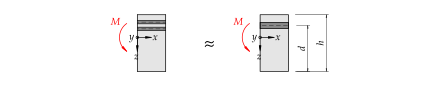
\includegraphics{index_files/mediabag/../images/QS_analyse_1.pdf}

}

\caption{\label{fig-qs_vereinfachung}Vereinfachung der Bewehrungsführung
des Plattenstreifens}

\end{figure}

Die Parameter aus der Tabelle~\ref{tbl-params_krummung} finden Einfluss
in die Berechnungen. Neben den Parametern wird das Stoffgesetz für den
Betonstahl in Abbildung~\ref{fig-stahlkennlinie} hinterlegt. Das
bilineare, bzw. linear-elastisch linear-plastische
Spannungs-Dehnungs-Diagramm für den Betonstahl hält den Rechenaufwand
klein und liefert eine ausreichende Genauigkeit.

\hypertarget{tbl-params_krummung}{}
\begin{longtable}[]{@{}
  >{\raggedright\arraybackslash}p{(\columnwidth - 2\tabcolsep) * \real{0.5000}}
  >{\raggedright\arraybackslash}p{(\columnwidth - 2\tabcolsep) * \real{0.5000}}@{}}
\caption{\label{tbl-params_krummung}Berechnungsparameter
Momenten-Krümmungs-Beziehung}\tabularnewline
\toprule\noalign{}
\begin{minipage}[b]{\linewidth}\raggedright
Parameter
\end{minipage} & \begin{minipage}[b]{\linewidth}\raggedright
\hspace{0pt}
\end{minipage} \\
\midrule\noalign{}
\endfirsthead
\toprule\noalign{}
\begin{minipage}[b]{\linewidth}\raggedright
Parameter
\end{minipage} & \begin{minipage}[b]{\linewidth}\raggedright
\hspace{0pt}
\end{minipage} \\
\midrule\noalign{}
\endhead
\bottomrule\noalign{}
\endlastfoot
\(E_{s} = \frac{200000.0 \text{N}}{\text{mm}^{2}}\) &
\(\oslash_{s} = 12.0 \text{mm}\) \\
\(c_{nom} = 20.0 \text{mm}\) &
\(f_{cc} = \frac{58.8 \text{N}}{\text{mm}^{2}}\) \\
\(f_{su} = \frac{630.3 \text{N}}{\text{mm}^{2}}\) &
\(f_{sy} = \frac{546.0 \text{N}}{\text{mm}^{2}}\) \\
\(s_{x} = 80.0 \text{mm}\) & \(\theta_{c3} = 30.0\) \\
\(\varepsilon_{cu} = 0.005\) & \(\varepsilon_{su} = 0.1117\) \\
\end{longtable}

Eine Berücksichtigung des verfestigenden Verhaltens ist essentiell, um
die Verformungen nach dem Fliessen des Betonstahls näherungsweise zu
bestimmen. Das Diagramm ist definiert bis zur Bruchdehnung
\(\varepsilon_{su}\) des Stahls. Das Verhalten gilt ebenso im negativen
Spannungs-Dehnungs Bereich.

\begin{figure}[H]

{\centering \includegraphics{index_files/mediabag/06_Versuch_2_A3_Jaeger_files/figure-pdf/fig-stahlkennlinie-output-1.pdf}

}

\caption{\label{fig-stahlkennlinie}Linear-elastisches,
linear-plastisches Spannungs-Dehnungs-Diagramm des Betonstahls}

\end{figure}

Dem Beton wird die Betonkennlinie, die in
Abbildung~\ref{fig-betonkennlinie} dargestellt ist, hinterlegt. Diese
zeigt ein linear-elastisches ideal-plastisches Verhalten. Im positiven
Bereich lässt sich die Betonspannung bis zur Betonzugfestigkeit
\(f_{ct}\) erhöhen, im negativen Spannungsbereich beginnt ein
Plastifizieren beim Erreichen der Betondruckfestigkeit \(f_c\). Dies ist
bis zur Bruchstauchung \(\varepsilon_{cu}\) definiert.

\begin{figure}[H]

{\centering \includegraphics{index_files/mediabag/06_Versuch_2_A3_Jaeger_files/figure-pdf/fig-betonkennlinie-output-1.pdf}

}

\caption{\label{fig-betonkennlinie}Linear-elastisches, ideal-plastisches
Spannungs-Dehnungs-Diagramm des Betons}

\end{figure}

\hypertarget{querschnittsanalyse}{%
\subsection{Querschnittsanalyse}\label{querschnittsanalyse}}

Basierend auf den eben beschriebenen Grundlagen wird folgend eine
Querschnittsanalyse durchgeführt. Dabei wird der Querschnitt vor dem
Reissen, nach dem Reissen, beim Fliessen der Zugbewehrung und beim
Versagen untersucht. Durch die Wahl aussagekräftiger Zustände im
Querschnitt lässt sich eine nicht-lineare Momenten-Krümmungs-Beziehung
mit überschaubarem Rechenaufwand ermitteln.

\hypertarget{schwerpunkt-des-querschnitts}{%
\subsubsection{Schwerpunkt des
Querschnitts}\label{schwerpunkt-des-querschnitts}}

Zunächst sind die Eigenschaften des Querschnitts zu bestimmen. Die
Bestimmung der Wertigkeit \(n\) ermöglicht die Betrachtung des
Querschnitts als homogenen Betonquerschnitt. Diese findet Einfluss bei
der Schwerpunktsbestimmung, sowie bei der Bestimmung des
Flächenträgheitmoments.

\begin{equation}n = \frac{E_{s}}{E_{c}}\end{equation}

\begin{equation}n = 5.14\end{equation}

Mithilfe der Querschnittsfläche der Zugstäbe unter Berücksichtigung der
Wertigkeit sowie der Betonquerschnittsfläche, lässt sich eine ideelle
Querschnittsfläche ermitteln. Die Querschnittsfläche der Zugstäbe ist
die folgende:

\begin{equation}A_{s} = 2 b \frac{\pi \oslash_{s}^{2}}{4 s_{x}}\end{equation}

\begin{equation}A_{s} = 2262.0 \text{mm}^{2}\end{equation}

Die Betonquerschnittsfläche hingegen beträgt:

\begin{equation}A_{c} = b h\end{equation}

\begin{equation}A_{c} = 160000.0 \text{mm}^{2}\end{equation}

Und die ideelle Querschnittsfläche resultiert zu:

\begin{equation}A_{i} = A_{c} + A_{s} \left(n - 1\right)\end{equation}

\begin{equation}A_{i} = 169372.0 \text{mm}^{2}\end{equation}

Der vertikale Abstand von der Oberkante zum Schwerpunkt, aufgezeigt in
der Abbildung~\ref{fig-qs_a3}, beträgt:

\begin{equation}\zeta_{c} = \frac{\frac{A_{c} h}{2} + A_{s} \left(1.5 \oslash_{s} + c_{nom}\right) \left(n - 1\right)}{A_{i}}\end{equation}

\begin{equation}\zeta_{c} = 96.6 \text{mm}\end{equation}

\hypertarget{fluxe4chentruxe4gheitsmoment}{%
\subsubsection{Flächenträgheitsmoment}\label{fluxe4chentruxe4gheitsmoment}}

Als weitere Querschnittseigenschaft gilt es das Flächenträgheitsmoment
zu berechnen. Dieses wird ebenfalls am ideellen Querschnitt bestimmt.
Die Eigenträgheitsmomente der Kreisquerschnitte der Stäbe sind nicht
berücksichtigt. Da deren Einfluss vernachlässigbar klein ist. Lediglich
der Steiner-Anteil fliesst in die Berechnung ein:

\begin{equation}I^{I} = A_{s} \left(n - 1\right) \left(\frac{3 \oslash_{s}}{2} + c_{nom} - \zeta_{c}\right)^{2} + \frac{b h^{3}}{12} + b h \left(\frac{h}{2} - \zeta_{c}\right)^{2}\end{equation}

\begin{equation}I^{I} = 5.67 \cdot 10^{8} \text{mm}^{4}\end{equation}

\hypertarget{ungerissen---zustand-1}{%
\subsubsection{Ungerissen - Zustand 1}\label{ungerissen---zustand-1}}

Der Zustand 1 betrachtet den Querschnitt unter Biegung vor dem Erreichen
der Betonzugfestigkeit. Durch das durchwegs elastische Verhalten kann
die Biegesteifigkeit anhand des Elastizitätmoduls des Betons und des
Flächenträgheitmoments des ideellen Querschnitts bestimmt werden.

\begin{equation}EI^{I} = E_{c} I^{I}\end{equation}

\begin{equation}EI^{I} = 2.206 \cdot 10^{4} \text{kN} \text{m}^{2}\end{equation}

Zugehörig zum Zustand 1 ist das Rissmoment. Das Rissmoment definiert den
Endpunkt des Zustands 1 im Momenten-Krümmungs-Diagramm, sprich beim
Erreichen der Zugfestigkeit des Betons. Dabei gilt die Modellierung
gemäss Abbildung~\ref{fig-qs2}. Die Spannung in den Zugstäben wird
vernachlässigt.

\begin{figure}[H]

{\centering 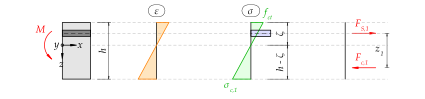
\includegraphics{index_files/mediabag/../images/QS_analyse_2.pdf}

}

\caption{\label{fig-qs2}Querschnittsanalyse vor dem Reissen des Betons}

\end{figure}

Die Betondruckspannung lässt sich anhand der über die Querschnittshöhe
linear verlaufenden Spannung bestimmen.

\begin{equation}\sigma_{c 1} = \frac{f_{ct} \left(h - \zeta_{c}\right)}{\zeta_{c}}\end{equation}

\begin{equation}\sigma_{c 1} = \frac{4.86 \text{N}}{\text{mm}^{2}}\end{equation}

Zur Bestimmung des Rissmoments gilt es den Hebelarm der inneren Kräfte
zu definieren:

\begin{equation}z_{1} = - 1.5 \oslash_{s} - c_{nom} + \frac{2 h}{3} + \frac{\zeta_{c}}{3}\end{equation}

\begin{equation}z_{1} = 128.0 \text{mm}\end{equation}

Die Betondruckkraft lässt sich anhand der Betondruckspannung und der
Betonfläche bestimmen:

\begin{equation}F_{c,1} = \frac{b \sigma_{c 1} \left(h - \zeta_{c}\right)}{2}\end{equation}

\begin{equation}F_{c,1} = 201.0 \text{kN}\end{equation}

Und das Rissmoment resultiert schliesslich zu:

\begin{equation}M_{r} = F_{c,1} z_{1}\end{equation}

\begin{equation}M_{r} = 25.63 \text{kN} \text{m}\end{equation}

Unter Berücksichtigung der Biegesteifigkeit lässt sich die Krümmung beim
Reissen des Querschnitts bestimmen.

\begin{equation}\chi_{r} = \frac{M_{r}}{EI^{I}}\end{equation}

\begin{equation}\chi_{r} = \frac{0.00116}{\text{m}}\end{equation}

\hypertarget{gerissen-elastisch---zustand-2}{%
\subsubsection{Gerissen elastisch - Zustand
2}\label{gerissen-elastisch---zustand-2}}

Mit dem Zustand 2 wird darauf abgezielt, den gerissenen Bereich im
Momenten-Krümmungs-Diagramm darzustellen. Der Querschnitt nach dem
Reissen ist in der Abbildung~\ref{fig-qs3} dargestellt. Der Betonstahl
hat die Fliessgrenze noch nicht erreicht. Der Beton hat ebenfalls seine
Druckfestigkeit noch nicht erreicht.

\begin{figure}[H]

{\centering 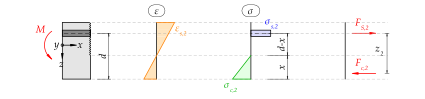
\includegraphics{index_files/mediabag/../images/QS_analyse_3.pdf}

}

\caption{\label{fig-qs3}Querschnittsanalyse nach dem Reissen des Betons}

\end{figure}

Mittels Gleichgewicht der Kräfte lässt sich die Betondruckzonenhöhe
bestimmen. Dazu wird zuerst die Beziehung zwischen der
Betonstahlspannung und der Betonstahlkraft dargestellt.

\begin{equation}F_{s,2} = A_{s} \sigma_{s 2}\end{equation}

Die Betonstahlspannung für linear elastisches Verhalten folgt zu:

\begin{equation}\sigma_{s 2} = E_{s} \varepsilon_{s2}\end{equation}

Die Betondruckkraft anhand des dreieckigen Verlaufs in
Abbildung~\ref{fig-qs3} beträgt:

\begin{equation}F_{c,2} = \frac{b \sigma_{c 2} x_{2}}{2}\end{equation}

Und die Betonspannung, ebenfalls bestimmt durch ein linear elastisches
Verhalten, ist definiert durch:

\begin{equation}\sigma_{c 2} = E_{c} \varepsilon_{c,2}\end{equation}

Anhand des Dehnungsverlaufs in Abbildung~\ref{fig-qs3} lässt sich die
Betondehnung bestimmen:

\begin{equation}\varepsilon_{c,2} = \frac{\varepsilon_{s2} x_{2}}{d - x_{2}}\end{equation}

Werden nun die horizontalen Kräfte gleichgesetzt, dargestellt in der
folgenden Beziehung:

\begin{equation}F_{c,2} = F_{s,2}\end{equation}

Und mit den bestimmten Gleichungen substituiert, sowie mit \(n\) und
\(\rho\) ersetzt, so folgt:

\begin{equation}n = \frac{E_{s}}{E_{c}}\end{equation}

\begin{equation}\rho = \frac{A_{s}}{b d}\end{equation}

\begin{equation}E_{s} b d \rho \varepsilon_{s2} = \frac{E_{s} b \varepsilon_{s2} x_{2}^{2}}{2 n \left(d - x_{2}\right)}\end{equation}

Aus welcher abschliessend die Betondruckzonenhöhe ermittelt werden kann:

\begin{equation}x_{2} = d \left(- n \rho + \sqrt{n \rho \left(n \rho + 2\right)}\right)\end{equation}

\begin{equation}x_{2} = 55.6 \text{mm}\end{equation}

Die hergeleiteten Beziehungen gelten für den gesamten gerissenen
Bereich. Mit der Wahl eines Biegemoments kann die Betonstahldehnung und
die erforderliche Krümmung bestimmt werden. Wird das in Zustand 1
ermittelte Rissmoment angesetzt, so lässt sich der Startpunkt des
gerissenen Bereichs im Momenten-Krümmungs-Diagramm bestimmen.

\begin{equation}M_{2} = F_{s,2} \left(d - \frac{x_{2}}{3}\right)\end{equation}

\begin{equation}M_{2} = M_{r}\end{equation}

\begin{equation}M_{r} = A_{s} E_{s} \varepsilon_{s2} \left(d - \frac{x_{2}}{3}\right)\end{equation}

Daraus resultiert die folgende Betonstahldehnung und die
Betonstahlspannung. Die in diesem Zustand ermittelte Betonstahlspannung
findet bei der Bestimmung der Rissweiten Einfluss, diese wird dort als
Rissspannung angesetzt.

\begin{equation}\varepsilon_{s2} = 0.000395\end{equation}

\begin{equation}\sigma_{s 2} = \frac{79.0 \text{N}}{\text{mm}^{2}}\end{equation}

Der Zustand 2 wird mit der Ermittlung der Krümmung und der
entsprechenden Biegesteifigkeit abgeschlossen. Die Krümmung kann anhand
des Dehnungsverlaufs in Abbildung~\ref{fig-qs3} ermittelt werden:

\begin{equation}\chi^{II} = \frac{\varepsilon_{s2}}{d - x_{2}}\end{equation}

\begin{equation}\chi^{II} = \frac{0.00371}{\text{m}}\end{equation}

Die gerissene Biegesteifigkeit folgt zu:

\begin{equation}EI^{II} = \frac{M_{2}}{\chi^{II}}\end{equation}

\begin{equation}EI^{II} = 6903.8 \text{kN} \text{m}^{2}\end{equation}

Mit dem Rissmoment und der Krümmung aus dem Zustand 2 ist der
Anfangspunkt für den gerissenen Zustand im Momenten-Krümmungs-Diagramm
definiert.

\hypertarget{fliessen-der-bewehrung---zustand-3}{%
\subsubsection{Fliessen der Bewehrung - Zustand
3}\label{fliessen-der-bewehrung---zustand-3}}

Der Zustand 3 entspricht dem Zustand 2. Einzig die Stahlspannung
erreicht die Fliessspannung. Dargestellt ist dies in der
Abbildung~\ref{fig-qs4} .

\begin{figure}[H]

{\centering \includegraphics{index_files/mediabag/../images/QS_analyse_4.pdf}

}

\caption{\label{fig-qs4}Querschnittsanalyse mit erreichter
Fliessspannung im Stab}

\end{figure}

Durch das Gleichgewicht der horizontalen Kräfte folgen die Beziehungen:

\begin{equation}\sigma_{c 3} = \frac{E_{c} f_{sy} x_{3}}{E_{s} \left(d - x_{3}\right)}\end{equation}

\begin{equation}A_{s} f_{sy} = \frac{b \sigma_{c 3} x_{3}}{2}\end{equation}

Welche durch das Auflösen die Druckzonenhöhe des Zustands 2 ergibt.

\begin{equation}x_{3} = \frac{- A_{s} E_{s} + \sqrt{A_{s} E_{s} \left(A_{s} E_{s} + 2 E_{c} b d\right)}}{E_{c} b}\end{equation}

\begin{equation}x_{3} = 55.6 \text{mm}\end{equation}

Daraus lässt sich das Fliessmoment bestimmen, welches den Endpunkt im
Momenten-Krümmungs-Diagramm für den gerissenen Zustand definiert:

\begin{equation}M_{y} = A_{s} f_{sy} \left(d - \frac{x_{3}}{3}\right)\end{equation}

\begin{equation}M_{y} = 177.2 \text{kN} \text{m}\end{equation}

Abschliessend lässt sich die Krümmung für den Zustand 3 bestimmen.

\begin{equation}\chi_{y} = \frac{\varepsilon_{sy}}{d - x_{3}}\end{equation}

\begin{equation}\chi_{y} = \frac{0.0257}{\text{m}}\end{equation}

\hypertarget{biegewiderstand---zustand-4}{%
\subsubsection{Biegewiderstand - Zustand
4}\label{biegewiderstand---zustand-4}}

Der Biegewiderstand des Querschnitts kann durch die Plastifizierung der
Betondruckzone bestimmt werden. Vereinfacht wird dem Betonstahl die
statische Zugfestigkeit vorausgesetzt, um das verfestigende Verhalten
annähernd abzubilden.

\begin{figure}[H]

{\centering \includegraphics{index_files/mediabag/../images/QS_analyse_5.pdf}

}

\caption{\label{fig-qs5}Querschnittsanalyse mit erreichter Zugfestigkeit
im Stab und plastifizierter Betondruckzone}

\end{figure}

Der Verlauf der Betonspannung wird mit einem rechteckigen Spannungsblock
idealisiert. Dazu wird die Druckzonenhöhe um den Faktor 0.85 reduziert.
Aus dem Gleichgewicht der horizontalen Kräfte folgt:

\begin{equation}A_{s} f_{su} = 0.85 b f_{c} x_{4}\end{equation}

Aus welcher sich die Druckzonenhöhe bestimmen lässt:

\begin{equation}x_{4} = 51.4 \text{mm}\end{equation}

Die Druckzonenhöhe definiert den Hebelarm der inneren Kräfte:

\begin{equation}z_{4} = d - 0.425 x_{4}\end{equation}

\begin{equation}z_{4} = 140.0 \text{mm}\end{equation}

Welche den Biegewiderstand definiert:

\begin{equation}M_{R} = A_{s} f_{su} z_{4}\end{equation}

\begin{equation}M_{R} = 199.8 \text{kN} \text{m}\end{equation}

Abschliessend gilt es die Krümmung und die Biegesteifigkeit zu
berechnen, sowie zu kontrollieren ob die Stahldehnung die Bruchdehnung
erreicht hat, bzw. nicht überschritten hat. Die Krümmung lässt sich
anhand der Betonstauchung ermitteln:

\begin{equation}\chi_{u} = \frac{\varepsilon_{cu}}{x_{4}}\end{equation}

\begin{equation}\chi_{u} = \frac{0.0974}{\text{m}}\end{equation}

Die Biegesteifigkeit im Bereich 3 beträgt:

\begin{equation}EI^{III} = \frac{M_{R}}{\chi_{u}}\end{equation}

\begin{equation}EI^{III} = 2.05 \cdot 10^{3} \text{kN} \text{m}^{2}\end{equation}

Die Betonstahldehnung lässt sich anhand des linearen Dehnungsverlaufs
und der Betonstauchung bestimmen:

\begin{equation}\varepsilon_{s4} = \frac{\varepsilon_{cu} \left(d - x_{4}\right)}{x_{4}}\end{equation}

\begin{equation}\varepsilon_{s4} = 0.0108\end{equation}

Die Bruchdehnung des Stahls wird nicht erreicht. Der Querschnitt versagt
im Druckbereich. Die Annahme, dem Betonstahl die statische Zugfestigkeit
zu Grunde zu legen ist grundsätzlich nicht gerechtfertig. Der Vergleich
mit den Versuchsergebnissen zeigt jedoch, dass sich diese Annahme
bewährt.

\begin{equation}\varepsilon_{su} = 0.1117\end{equation}

\hypertarget{momenten-kruxfcmmungs-diagramm}{%
\subsubsection{Momenten-Krümmungs-Diagramm}\label{momenten-kruxfcmmungs-diagramm}}

Folgend ist die Querschnittsanalyse in einem
Momenten-Krümmungs-Diagramm, aufgezeigt in der
Abbildung~\ref{fig-mchi_diagramm}, zusammengefasst. Die punktuellen
Bestimmungen der Krümmung und deren entsprechenden Biegemomente aus der
Querschnittsanalyse sind miteinander linear verbunden. Die nicht-lineare
Beziehung zwischen Moment und Krümmung ist erkennbar.

\begin{figure}[H]

{\centering 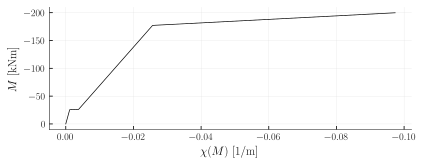
\includegraphics{index_files/mediabag/06_Versuch_2_A3_Jaeger_files/figure-pdf/fig-mchi_diagramm-output-1.pdf}

}

\caption{\label{fig-mchi_diagramm}Momenten-Krümmungs-Diagramm, definiert
durch die Querschnittsanalyse}

\end{figure}

Die erste Steigung im Diagramm beschreibt den ungerissenen Zustand 1.
Dieser hat die Neigung von \(EI^I\). Darauf folgt eine schlagartige
Erhöhung der Krümmung ohne Steigerung des Moments. Dies entspricht dem
Übergang vom gerissenen zum ungerissenen Zustand 2. Dabei steigt der
Verlauf mit der Neigung \(EI^{II}\) bis zum Fliessen der Bewehrung
(Zustand 3). Ab diesem Punkt erfolgt ein verfestigendes Verhalten des
Betonstahls und ein Plastifizieren der Betondruckzone bis zum Erreichen
des Biegewiderstands (Zustand 4).

\hypertarget{zustandslinien-der-kruxfcmmung}{%
\subsubsection{Zustandslinien der
Krümmung}\label{zustandslinien-der-kruxfcmmung}}

Die Momenten-Krümmungs-Beziehung wird nun zur Bestimmung des
Krümmungsverlaufs verwendet. Der Biegemomentenverlauf \(M(x)\), als
Eingabe in die Funktion der Krümmung \(\chi(M)\), führt zu den
Zustandslinien der Krümmung in Abbildung~\ref{fig-chi_x_diagramm}.
Dargestellt ist der Krümmungsverlauf exemplarisch für die Zustandslinien
der Biegemomente aus der Abbildung~\ref{fig-m_x}.

\begin{figure}[H]

{\centering \includegraphics{index_files/mediabag/06_Versuch_2_A3_Jaeger_files/figure-pdf/fig-chi_x_diagramm-output-1.pdf}

}

\caption{\label{fig-chi_x_diagramm}Krümmungsverlauf entlang der
Stabachse}

\end{figure}

Über dem Auflager \(C\) ist für die dargestellte Laststufe der
Biegewiderstand erreicht. Man befindet sich im Endbereich der
Momenten-Krümmungs-Beziehung. Ebenfalls ersichtlich ist der sprunghafte
Übergang zwischen dem ungerissenen und dem gerissenen Bereich.

\hypertarget{punktuelle-bestimmung-der-verformung}{%
\subsubsection{Punktuelle Bestimmung der
Verformung}\label{punktuelle-bestimmung-der-verformung}}

Unter Anwendung der Arbeitsgleichung kann die Verformung nach
Gleichung~\ref{eq-arbeitsgleichung} bestimmt werden. Die Position der
fiktiven Einwirkung entspricht der Position der berechneten Verformung.
Folglich ist an der Stelle \(x=0.11\) eine Einzellast \(\bar{F} = 1\)
angesetzt, was zum virtuellen Biegemomentenverlauf in der
Abbildung~\ref{fig-m_x_diagramm_virtuell} führt.

\begin{figure}[H]

{\centering \includegraphics{index_files/mediabag/06_Versuch_2_A3_Jaeger_files/figure-pdf/fig-m_x_diagramm_virtuell-output-1.pdf}

}

\caption{\label{fig-m_x_diagramm_virtuell}Biegemomentenverlauf für den
virtuellen Kräftezustand}

\end{figure}

Für die maximale Last beträgt die Deformation an der Stelle \(w_1\)
beispielsweise:

\begin{equation}w_{1} = 15.3 \text{mm}\end{equation}

\hypertarget{zugversteifung}{%
\subsection{Zugversteifung}\label{zugversteifung}}

Folgend wird die Modellbildung nach Marti aus dem
Kapitel~\ref{sec-zuggurtmodell} angewendet. Die bisherige Betrachtung
beschränkt sich auf einen schlagartigen Wechsel von ungerissen zu
vollständig gerissen. Dabei wird der Bereich zwischen den Rissen
ebenfalls als gerissen angenommen. Mittels der Zugversteifung wird ein
theoretischer Rissabstand ermittelt und zwischen den Rissen eine
versteifte Wirkung zwischen Betonstahl und Beton angenommen
(Verbundwirkung). Die Krümmungsdifferenz beträgt:

\begin{equation}\Delta\chi{\left(\lambda \right)} = \frac{\lambda}{2} \frac{f_{ct} \left(1 - \rho_{eff}\right)}{E_{s} \rho_{eff} \left(d - x_{2}\right)}\end{equation}

\begin{equation}\Delta\chi{\left(\lambda \right)} = \frac{0.00131 \lambda}{\text{m}}\end{equation}

Der mechanische Bewehrungsgehalt beschreibt sich zu:

\begin{equation}\rho_{eff} = \frac{1}{- n + 1 + \frac{E_{s} M_{r} \left(d - x_{2}\right)}{EI^{II} f_{ct}}}\end{equation}

\begin{equation}\rho_{eff} = 0.0753\end{equation}

Eine Abschätzung des Rissabstands ist folgend gezeigt. Dabei sind die
Resultate für \(\lambda = 1\) und \(\lambda = 0.5\) berechnet.

\begin{equation}s_{rm} = \frac{\oslash_{s} \lambda \left(1 - \rho_{eff}\right)}{4 \rho_{eff}}\end{equation}

\begin{equation}s_{rm} = 36.8 \text{mm}\end{equation}

\begin{equation}s_{rm} = 18.4 \text{mm}\end{equation}

Die Rissbreite ist abhängig von der Betonstahlspannung. Da vor dem
Reissen des Betons keine Risse vorhanden sind, darf die Rissspannung von
der Betonstahlspannung subtrahiert werden. Die Rissspannung lässt sich
anhand der Betonstahlkraft aus dem Zustand 2 bestimmen.

\begin{equation}\sigma_{sr0} = \frac{F_{s,2}}{A_{s}}\end{equation}

Die Bestimmung der Rissbreite ist folgend gezeigt. Für die Stahlspannung
wird die Fliessspannung eingesetzt. Die Variation des Parameters
\(\lambda = 1 ; 0.5\) gilt hier ebenfalls.

\begin{equation}w_{r} = \frac{s_{rm} \left(- \lambda \sigma_{sr0} + 2 \sigma_{sr}\right)}{2 E_{s}}\end{equation}

\begin{equation}w_{r} = 0.0933 \text{mm}\end{equation}

\begin{equation}w_{r} = 0.0485 \text{mm}\end{equation}

Die Resultate sind vergleichbar mit den gemessenen Rissbreiten der
Laststufe 12, die in {[}\protect\hyperlink{ref-Jaeger2006}{1}{]}
dargestellt sind. Diese liegen in einem Wertebereich von
\(0.15 \text{ mm}\) bis \(0.3 \text{ mm}\). Die Rissweiten werden
folglich unterschätzt.

Der Einfluss der Zugversteifung lässt sich direkt im
Momenten-Krümmungs-Diagramm darstellen. Unter Berücksichtigung der
beiden \(\lambda\)-Grenzwerte ist der Einfluss der Zugversteifung in
Abbildung~\ref{fig-mchi_diagramm_zugversteifung} gezeigt.

\begin{figure}[H]

{\centering \includegraphics{index_files/mediabag/06_Versuch_2_A3_Jaeger_files/figure-pdf/fig-mchi_diagramm_zugversteifung-output-1.pdf}

}

\caption{\label{fig-mchi_diagramm_zugversteifung}Momenten-Krümmungs-Diagramm
mit Zugversteifung}

\end{figure}

Es zeigt sich ein steiferes Verhalten im gerissenen Bereich. Der
Einfluss ist relativ gering.

\hypertarget{fachwerksanalyse}{%
\section{Fachwerksanalyse}\label{fachwerksanalyse}}

Abschliessend wird das Modell aus dem Kapitel~\ref{sec-fachwerk} auf den
Versuch angewendet. Die bisherigen Analysen beschränken sich auf eine
Querschnittsbetrachtung. Der Kraftfluss lässt sich mit einem
Spannungsfeld detaillierter verfolgen. Eine Einteilung in Parallelfelder
und nicht-zentrierte Fächer ist in
Abbildung~\ref{fig-spannungsfelder_flach} gezeigt.

\begin{figure}[H]

{\centering \includegraphics{index_files/mediabag/../images/Spannungsfelder_flach.pdf}

}

\caption{\label{fig-spannungsfelder_flach}Plattenstreifen mit
Spannungsfeldern entsprechend dem Kraftfluss}

\end{figure}

Der Neigungswinkel der Betondruckstrebe wird in Anlehnung an die
Gleichung~\ref{eq-v_rds_sia262} zur Bestimmung des Querkraftwiderstands
von vertikaler Schubbewehrung, gemäss Ziffer 4.3.3.4.3
{[}\protect\hyperlink{ref-SIA2013a}{6}{]}, bestimmt. Dabei wird die
Querschnittsfläche der Schubbewehrung bestimmt.

\begin{equation}A_{s w} = 197.9 \text{mm}^{2}\end{equation}

Der Hebelarm der inneren Kräfte des Zustands 4 wird angesetzt.

\begin{equation}z_{4} = 140.0 \text{mm}\end{equation}

Die Fliessspannung wird mit der Zugfestigkeit \(f_{su}\) substituiert.
Dies gewährleistet, dass die Schubbewehrung den elastischen Bereich
verlässt. Der Querkraftwiderstand wird mit der maximal im System
auftretenden Querkraft ersetzt. Abschliessend gilt
\(\alpha = \theta_{c3}\). Dies führt zu folgendem Neigungswinkel:

\begin{equation}\theta_{c3,min} = \operatorname{acot}{\left(\frac{V_{R,s} s_{w}}{A_{s w} f_{su} z_{4}} \right)}\end{equation}

\begin{equation}\theta_{c3,min} = 0.599\end{equation}

\begin{equation}\theta_{c3,min} = 34.3 ^\circ\end{equation}

Der gewählte Neigungswinkel der Felder in der
Abbildung~\ref{fig-spannungsfelder_flach} orientiert sich an dem
berechneten Winkel. Ausserdem wurde darauf geachtet, dass alle Felder
parallel zueinander angeordnet sind.

Durch das Zusammenfassen der Felder zu Stäben resultiert das Fachwerk in
Abbildung~\ref{fig-fachwerk_flach}. Um aus dem Fachwerkmodell
zutreffende Verformungen zu ermitteln, gilt es den Pendelstäben passende
Dehnsteifigkeiten zuzuordnen.

\begin{figure}[H]

{\centering 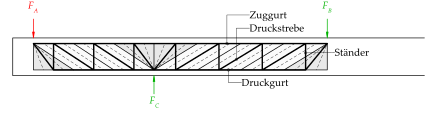
\includegraphics{index_files/mediabag/../images/Fachwerk_flach.pdf}

}

\caption{\label{fig-fachwerk_flach}Plattenstreifen mit Fachwerk durch
das Zusammenfassen der Spannungsfelder}

\end{figure}

Dem Zuggurt ist die Spannungs-Dehnungs-Beziehung gemäss
Abbildung~\ref{fig-stahlkennlinie} hinterlegt, sowie entspricht die
Querschnittsfläche jener der Zugbewehrung.

Die Querschnittsfläche des Druckgurts entspricht der Höhe des
plastischen Spannungsblocks des Zustands 4 multipliziert mit der
Plattenstreifenbreite. Diese wird als konstant über sämtliche Stäbe des
Druckgurtes angenommen. Des Weiteren ist die
Spannungs-Dehnungs-Beziehung gemäss Abbildung~\ref{fig-betonkennlinie}
angewendet.

Die Querschnittsfläche der Druckstreben entspricht der Streifenbreite
multipliziert mit der Parallelfeldbreite, gezeigt in
Abbildung~\ref{fig-spannungsfelder_flach}. Für die Diagonalen der nicht
zentrierten Fächer ist vereinfacht die gleiche Querschnittsfläche
hinterlegt. Dazu gilt die Spannungs-Dehnungs-Beziehung gemäss
Abbildung~\ref{fig-betonkennlinie}.

Die Ständer bilden die Schubbewehrung ab. Die Querschnittsfläche
resultiert aus der Anzahl an Schubdübeln im entsprechenden
Spannungsfeld. Es gilt die Spannungs-Dehnungs-Beziehung gemäss
Abbildung~\ref{fig-stahlkennlinie}. Die
Abbildung~\ref{fig-schubbew_fw_flach} zeigt, dass pro Ständer drei
Schubdübel umfasst sind.

\begin{figure}[H]

{\centering 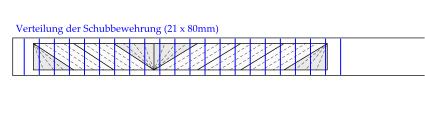
\includegraphics{index_files/mediabag/../images/Schubbewehrung_aufteilung_flach.pdf}

}

\caption{\label{fig-schubbew_fw_flach}Plattenstreifen mit dargestellter
Schubbewehrung und Spannungsfeldern}

\end{figure}

Mit der definierten Geometrie und den entsprechenden Steifigkeiten
resultieren die Verformungen für die Maximallast zu
\(175.2 \text{ mm}\), aufgezeigt in der
Abbildung~\ref{fig-deformation_fw}.

\begin{figure}[H]

{\centering 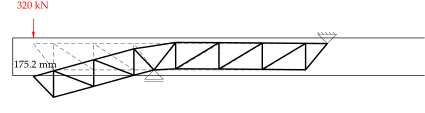
\includegraphics{index_files/mediabag/../images/Def_Fachwerk.pdf}

}

\caption{\label{fig-deformation_fw}Plattenstreifen mit verformten
Fachwerk}

\end{figure}

\hypertarget{modellvergleich}{%
\section{Modellvergleich}\label{modellvergleich}}

Abgeschlossen wird die Analyse des Dreipunktbiegeversuchs mit einer
Gegenüberstellung der angewendeten Methoden. Der Fokus liegt auf dem
Vergleich der experimentell ermittelten Verformungen und den
Verformungen aus den Modellen.

\hypertarget{kruxfcmmung}{%
\subsection{Krümmung}\label{kruxfcmmung}}

Der Modellvergleich wird bei der Beschreibung der Krümmung der
unterschiedlichen Modelle gestartet. Aus dem Vergleich der
Momenten-Krümmungs-Beziehung, dargestellt in
Abbildung~\ref{fig-mchi_diagramm_vergleich}, lassen sich die
Biegesteifigkeiten herauslesen.

\begin{figure}[H]

{\centering \includegraphics{index_files/mediabag/06_Versuch_2_A3_Jaeger_files/figure-pdf/fig-mchi_diagramm_vergleich-output-1.pdf}

}

\caption{\label{fig-mchi_diagramm_vergleich}Momenten-Krümmungs-Diagramm
zum Vergleich der unterschiedlichen Modelle}

\end{figure}

Die Unterschiede des Detaillierungsgrad der Beziehung zwischen den
Modellen ist deutlich erkennbar. Ebenso ersichtlich ist der geringe
Einfluss der Zugversteifung auf die Biegesteifigkeit.

Die Abbildung~\ref{fig-chi_x_diagramm_vergleich} zeigt den
Krümmungsverlauf für den Biegemomentenverlauf aus
Abbildung~\ref{fig-m_x}. Ausgehend davon, dass die nicht-lineare
Momenten-Krümmungs-Beziehung den effektiven Krümmungsverlauf präzise
abbilden kann, zeigen die konstanten Biegesteifigkeiten deutliche
Abweichungen. Der Fliessbereich über dem Auflager \(C\) kann nicht
abgebildet werden. Des Weiteren zeigt sich ein ausgeprägter gerissener
Bereich, welcher mit der konstanten ungerissenen Biegesteifigkeit als
deutlich zu steif eingeschätzt wird.

\begin{figure}[H]

{\centering \includegraphics{index_files/mediabag/06_Versuch_2_A3_Jaeger_files/figure-pdf/fig-chi_x_diagramm_vergleich-output-1.pdf}

}

\caption{\label{fig-chi_x_diagramm_vergleich}Krümmungsverlauf, mit
unterschiedlichen Modellen ohne Versatzmass}

\end{figure}

Das analoge Vorgehen gilt für den Biegemomentenverlauf mit dem
Versatzmass aus Abbildung~\ref{fig-m_x_versatz}. Dargestellt ist der
Krümmungsverlauf für diesen in
Abbildung~\ref{fig-chi_x_diagramm_laengszugkraft}.

\begin{figure}[H]

{\centering \includegraphics{index_files/mediabag/06_Versuch_2_A3_Jaeger_files/figure-pdf/fig-chi_x_diagramm_laengszugkraft-output-1.pdf}

}

\caption{\label{fig-chi_x_diagramm_laengszugkraft}Krümmungsverlauf, mit
unterschiedlichen Modellen mit Versatzmass}

\end{figure}

Die Schwächen der konstanten Biegesteifigkeiten zeigen sich hier
ebenfalls. Auffallend dabei ist der deutlich breitere Fliessbereich aus
der nicht-linearen Momenten-Krümmungs-Beziehung. Die Verformung
resultiert, wie in Gleichung~\ref{eq-arbeitsgleichung} beschrieben, aus
der Integration des Krümmungsverlaufs. Folglich hat die Verbreiterung im
Fliessbereich einen signifikanten Einfluss auf die Verformung.

\hypertarget{verformung}{%
\subsection{Verformung}\label{verformung}}

Ein direkter Vergleich der Verformungen mit den gemessenen
Versuchsresultaten ermöglicht die Erstellung von
Last-Verformungs-Diagrammen. Dazu sind für die beschriebenen Modelle die
Verformungen für sämtliche Laststufen bestimmt worden. In
Abbildung~\ref{fig-last_verformung_vergleich} und
Abbildung~\ref{fig-last_verformung_laengszug} sind diese für die
Biegemomentenverläufe aus der Abbildung~\ref{fig-m_x} und der
Abbildung~\ref{fig-m_x_versatz} gezeigt. Welche sich in der
Berücksichtigung des Versatzmasses unterscheiden. Die Verformung ist an
der Stelle \(w_1\) gemessen, dargestellt ist die Position in der
Abbildung~\ref{fig-system_2_lager}.

\begin{figure}[H]

{\centering 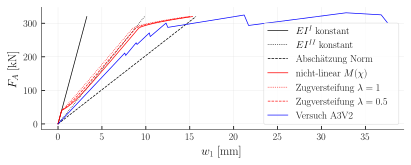
\includegraphics{index_files/mediabag/06_Versuch_2_A3_Jaeger_files/figure-pdf/fig-last_verformung_vergleich-output-1.pdf}

}

\caption{\label{fig-last_verformung_vergleich}Last-Verformungs-Diagramm
an der Stelle \(w_1\) ohne Versatzmass}

\end{figure}

Es zeigt sich, dass mit einer konstanten ungerissenen Biegesteifigkeit
die Verformungen nicht zufriedenstellend abbildbar sind. Bereits im
gerissenen Bereich zeigen sich deutliche Abweichungen zu den
Versuchsmessungen. Die Abweichungen sind für sämtliche Laststufen
deutlich. Mit einer konstanten gerissenen Biegesteifigkeit nähert man
sich den Versuchsergebnissen an. Die Differenzen zu den
Versuchsmessungen steigen mit steigender Laststufe. Dies ist auf die
fehlende Modellierung des Fliessbereichs zurückzuführen. Zudem werden
die Verformungen für sämtliche Laststufen leicht unterschätzt. Die
Darstellung der Normabschätzung zeigt eine konservative Abschätzung der
Verformungen. Die Verformungen werden für sämtliche Laststufen bis zum
Erreichen des Fliessbereichs überschätzt. Bei der Berücksichtigung der
nicht-linearen Momenten-Krümmungs-Beziehung (in rot dargestellt), lässt
sich das Verformungsverhalten des Versuchs annähernd abbilden. Das
Modell bildet ein zu steifes Verhalten ab. Die Zugversteifung wirkt der
Modellgenauigkeit entgegen. Sowie zeigen sich deutliche Abweichungen im
Bereich der Traglast.

\begin{figure}[H]

{\centering 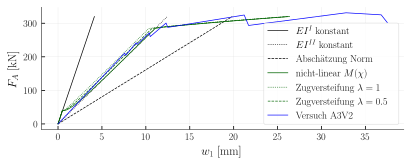
\includegraphics{index_files/mediabag/06_Versuch_2_A3_Jaeger_files/figure-pdf/fig-last_verformung_laengszug-output-1.pdf}

}

\caption{\label{fig-last_verformung_laengszug}Last-Verformungs-Diagramm
an der Stelle \(w_1\) mit Versatzmass}

\end{figure}

Die Abbildung~\ref{fig-last_verformung_laengszug} zeigt sämtliche
Berechnungsmethoden unter Berücksichtigung der Längszugkraft aus der
Querkraft, sprich dem Versatzmass. Die konstante Biegesteifigkeiten
zeigen die gleichen Mängel wie bei einer Nichtberücksichtigung des
Versatzmass. Ebenfalls zeigt die Normabschätzung eine deutliche
Überschätzung der Verformungen bis zum Erreichen der Fliessgrenze im
Betonstahl. Die Verformungen mittels der nicht-linearen
Momenten-Krümmungs-Beziehung zeigen eine präzise Übereinstimmung mit den
Versuchsmessungen. Einzig unter der Höchstlast ist eine Abweichung
vorhanden. Das Ergebnis ist jedoch vollumfänglich zufriedenstellend.
Abschliessend lässt sich festhalten, dass die Berücksichtigung des
Versatzmass zu einem weicheren Systemverhalten führt.

Folgend sind die Verformungen aus dem Fachwerkmodell dargestellt. Durch
die Aufteilung der Traganteile in die einzelnen Fachwerkstäbe lassen
sich Verformungsanteile aus der Schubbewehrung, der Gurte und der
Betondruckstreben gesondert ermitteln. Beispielsweise lässt sich der
Anteil der Schubbewehrung durch das Setzen der Steifigkeit der übrigen
Stäbe auf ein infinit grosses Mass bestimmen. Dargestellt ist dies in
Abbildung~\ref{fig-last_verformung_fachwerk}.

\begin{figure}[H]

{\centering \includegraphics{index_files/mediabag/06_Versuch_2_A3_Jaeger_files/figure-pdf/fig-last_verformung_fachwerk-output-1.pdf}

}

\caption{\label{fig-last_verformung_fachwerk}Last-Verformungs-Diagramm
an der Stelle \(w_1\) mit Fachwerksmodell, Fachwerkshöhe von 140 mm}

\end{figure}

Das Fachwerkmodell beschreibt den Verlauf bis zum Fliesspunkt der
Zugbewehrung ausreichend präzise. Die maximale Verformung jedoch, die
mit der rechnerisch ermittelten Höhe, sprich dem Hebelarm der inneren
Kräfte aus der Querschnittsanalyse, erzielt wird, überschreitet das Ziel
bei Weitem. Des Weiteren zeigt sich, dass die Verformung primär aus dem
Zuggurt resultiert. Die Schubbewehrung, Druckstrebe und der Druckgurt
haben einen vernachlässigbaren Einfluss.

Das Fachwerkmodell reagiert äusserst sensibel auf die gewählte Höhe.
Basierend auf dieser Tatsache ist in
Abbildung~\ref{fig-last_verformung_fachwerk_z_var} der
Verformungsverlauf mit der Anpassung der Fachwerskhöhe auf
\(160\text{ mm}\) gezeigt. Diese wurde nicht rechnerisch ermittelt, bzw.
wurde diese mittels Iteration bis zum Erreichen des passenden Verlaufs
bestimmt.

\begin{figure}[H]

{\centering 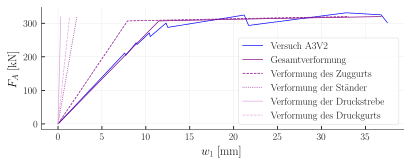
\includegraphics{index_files/mediabag/06_Versuch_2_A3_Jaeger_files/figure-pdf/fig-last_verformung_fachwerk_z_var-output-1.pdf}

}

\caption{\label{fig-last_verformung_fachwerk_z_var}Last-Verformungs-Diagramm
an der Stelle \(w_1\) mit Fachwerksmodell, Fachwerkshöhe von 160 mm}

\end{figure}

Das Modell mit der angepassten Höhe beschreibt den Verformungsverlauf
vollumfänglich präzise. Die Verformungsanteile aus der Schubbewehrung,
dem Druckgurt und der Druckstrebe sind auch hier nicht signifikant.

\bookmarksetup{startatroot}

\hypertarget{sec-vierpunkt}{%
\chapter{Vierpunktbiegeversuch}\label{sec-vierpunkt}}

Dieses Kapitel zeigt alle in Kapitel~\ref{sec-modellbeschrieb}
aufgezeigten Modelle, angewendet auf einen Vierpunktbiegeversuch. Das
Vorgehen ist in grossen Teilen analog dem Berechnungsvorgehen aus dem
Kapitel~\ref{sec-dreipunkt}. Es wird das Ziel verfolgt, die
Anwendbarkeit des Berechnungsapparats an einem weiteren Versuch zu
verifizieren, bzw. die Differenzen zwischen den mit den verschiedenen
Modellen berechneten Verformungen und den gemessenen Verformungen
aufzuzeigen.

\hypertarget{versuchsbeschreibung-1}{%
\section{Versuchsbeschreibung}\label{versuchsbeschreibung-1}}

Entnommen ist der Versuch SV14 aus
{[}\protect\hyperlink{ref-Tue2019}{2}{]}. Es handelt sich um einen
Vierpunktbiegeversuch. Es wird das Verhalten in Feldmitte analysiert. Im
Zugbereich sind Bewehrungsstäbe mit hochfestem Stahl verlegt. Die
Schubbewehrung ist minimal gehalten, sowie unterscheidet sich die
Teilung im linken und rechten Bereich des Balkens. Die Bewehrung ist
stets orthogonal oder parallel zu den Bauteilkanten verlegt. Dargestellt
ist dies in Abbildung~\ref{fig-system_sv14}.

\begin{figure}[H]

{\centering \includegraphics{index_files/mediabag/../images/versuchsskizze_14.pdf}

}

\caption{\label{fig-system_sv14}Lagerung und Belastung des Balkens,
nachgezeichnet nach {[}\protect\hyperlink{ref-Tue2019}{2}{]}}

\end{figure}

Das statische System entspricht einem einfachen Balken. Die Last wird an
beiden Angriffspunkten zeit- und betragsgleich eingeleitet. Gemäss den
Versuchsdaten tritt ein Biegeversagen bei einer Laststufe von
\(105 \text{ kN}\) ein.

\begin{figure}[H]

{\centering \includegraphics{index_files/mediabag/../images/verformungsverlauf_tue.pdf}

}

\caption{\label{fig-last_verformung_sv14}Last-Verformungs-Verlauf des
Balkens, entnommen aus {[}\protect\hyperlink{ref-Tue2019}{2}{]}}

\end{figure}

Das Last-Verformungs-Verhalten ist in der
Abbildung~\ref{fig-last_verformung_sv14} dargestellt.

\hypertarget{eigenschaften-der-baustoffe-1}{%
\section{Eigenschaften der
Baustoffe}\label{eigenschaften-der-baustoffe-1}}

Die Eigenschaften des hochfesten Betonstahls sind aus
{[}\protect\hyperlink{ref-annahutte_broschure}{10}{]} entnommen. Für den
Bst 550 sind Eigenschaften gemäss dem B500B aus der Schweizer Norm
{[}\protect\hyperlink{ref-SIA2013a}{6}{]} angesetzt mit einer Erhöhung
der Fliessgrenze auf \(550 \text{ N}/\text{mm}^2\). Lediglich die
Betondruckfestigkeit ist im Versuchsbericht
{[}\protect\hyperlink{ref-Tue2019}{2}{]} beschrieben. Diese wird als
Zielfestigkeit \(f_c = 35 \text{ N}/\text{mm}^2\) deklariert. Die
Zylinderdruckfestigkeit, sowie Zugefestigkeit und Elastizitätsmodul sind
folgend rechnerisch ermittelt. Die Zylinderdruckfestigkeit ist
entsprechend gewählt, um die Zielfestigkeit zu erreichen:

\begin{equation}f_{c} = 2.7 f_{cc}^{\frac{2}{3}}\end{equation}

\begin{equation}f_{c} = \frac{35.0 \text{N}}{\text{mm}^{2}}\end{equation}

Die Zugfestigkeit berechnet mittels der Gleichung nach
{[}\protect\hyperlink{ref-Jaeger2013}{9}{]} folgt zu:

\begin{equation}f_{ct} = 0.3 f_{cc}^{\frac{2}{3}}\end{equation}

\begin{equation}f_{ct} = \frac{3.89 \text{N}}{\text{mm}^{2}}\end{equation}

Die Abschätzung für den Elastizitätsmodul nach
{[}\protect\hyperlink{ref-Jaeger2013}{9}{]} resultiert zu:

\begin{equation}E_{c} = 10000 \sqrt[3]{f_{cc}}\end{equation}

\begin{equation}E_{c} = \frac{36011.0 \text{N}}{\text{mm}^{2}}\end{equation}

\hypertarget{reiner-biegetruxe4ger-1}{%
\section{Reiner Biegeträger}\label{reiner-biegetruxe4ger-1}}

Die beschriebenen Beziehungen aus dem Kapitel~\ref{sec-kontinua} sind
folgend auf den Versuch angewendet. Es sind Auflagerkräfte, sowie
elastische Zustandslinien der Schnittkräfte dargestellt. Als Grundlage
dient das statischen System in der
Abbildung~\ref{fig-stat_system_14_auflagerbreite}.

\begin{figure}[H]

{\centering \includegraphics{index_files/mediabag/../images/statisches_system_auflagerbreite_14.pdf}

}

\caption{\label{fig-stat_system_14_auflagerbreite}Statisches System des
Balkens mit berücksichtigter Auflagerbreite}

\end{figure}

\hypertarget{tbl-params_reiner_biegetraeger_sv14}{}
\begin{longtable}[]{@{}
  >{\raggedright\arraybackslash}p{(\columnwidth - 2\tabcolsep) * \real{0.5000}}
  >{\raggedright\arraybackslash}p{(\columnwidth - 2\tabcolsep) * \real{0.5000}}@{}}
\caption{\label{tbl-params_reiner_biegetraeger_sv14}Berechnungsparameter
der Systemgeometrie}\tabularnewline
\toprule\noalign{}
\begin{minipage}[b]{\linewidth}\raggedright
Parameter
\end{minipage} & \begin{minipage}[b]{\linewidth}\raggedright
\hspace{0pt}
\end{minipage} \\
\midrule\noalign{}
\endfirsthead
\toprule\noalign{}
\begin{minipage}[b]{\linewidth}\raggedright
Parameter
\end{minipage} & \begin{minipage}[b]{\linewidth}\raggedright
\hspace{0pt}
\end{minipage} \\
\midrule\noalign{}
\endhead
\bottomrule\noalign{}
\endlastfoot
\(a_{1} = 0.2 \text{m}\) & \(a_{2} = 1.5 \text{m}\) \\
\(a_{3} = 1.0 \text{m}\) & \(a_{4} = 1.5 \text{m}\) \\
\(a_{5} = 0.2 \text{m}\) & \(b = 170.0 \text{mm}\) \\
\(b_{Auflager} = 100 \text{mm}\) & \(h = 450.0 \text{mm}\) \\
\end{longtable}

\hypertarget{auflagerkruxe4fte-1}{%
\subsection{Auflagerkräfte}\label{auflagerkruxe4fte-1}}

Die Auflagerkräfte lassen sich anhand der Gleichgewichtsbeziehungen am
statisch bestimmten System ermitteln. Die Bestimmung derer ist für den
einfachen Balken trivial und entsprechen im Betrag den angreifenden
Kräften. In Anlehnung an das Vorgehen beim Dreipunktbiegeversuch im
Kapitel~\ref{sec-dreipunkt} ist folgend eine Ermittlung durch die
Gleichgewichtsbeziehungen gezeigt. Dazu wird zuerst die Gesamtlänge des
Balkens berechnet. Dies dient als Kontrollgrösse.

\begin{equation}l_{tot} = a_{1} + a_{2} + a_{3} + a_{4} + a_{5}\end{equation}

\begin{equation}l_{tot} = 4.4 \text{m}\end{equation}

Mittels dem Gleichgewicht der Momente um die Auflagerpunkte \(C\) und
\(B\) folgen die Beziehungen zwischen den Einwirkungen und den
Reaktionskräften:

\begin{equation}0 = - F_{A} a_{2} - F_{A} \left(a_{2} + a_{3}\right) - F_{C} \left(a_{2} + a_{3} + a_{4}\right)\end{equation}

\begin{equation}0 = F_{A} a_{4} + F_{A} \left(a_{3} + a_{4}\right) - F_{B} \left(a_{2} + a_{3} + a_{4}\right)\end{equation}

Werden diese nach den Reaktionskräften aufgelöst, folgen die
Beziehungen:

\begin{equation}F_{B} = \frac{F_{A} a_{3} + 2 F_{A} a_{4}}{a_{2} + a_{3} + a_{4}}\end{equation}

\begin{equation}F_{C} = \frac{- 2 F_{A} a_{2} - F_{A} a_{3}}{a_{2} + a_{3} + a_{4}}\end{equation}

Die Reaktionskräfte dividiert durch die Auflagerbreite resultieren zu
den folgenden Streckenlasten, bzw. Reaktionen:

\begin{equation}f_{B} = \frac{F_{A} a_{3} + 2 F_{A} a_{4}}{b_{Auflager} \left(a_{2} + a_{3} + a_{4}\right)}\end{equation}

\begin{equation}f_{C} = \frac{- 2 F_{A} a_{2} - F_{A} a_{3}}{b_{Auflager} \left(a_{2} + a_{3} + a_{4}\right)}\end{equation}

\begin{equation}f_{A} = \frac{F_{A}}{b_{Auflager}}\end{equation}

\hypertarget{zustandslinien-1}{%
\subsection{Zustandslinien}\label{zustandslinien-1}}

Folgend wird anhand der Einwirkung die Zustandslinien der Schnittkräfte
bestimmt. Dabei ist zu beachten, dass die Zustandslinien lediglich für
die maximal gewählte Laststufe gelten. Der Verlauf der Einwirkungen ist
in Abbildung~\ref{fig-q_x_sv14} aufgezeigt.

\begin{figure}[H]

{\centering \includegraphics{index_files/mediabag/07_Versuch_SV_14_files/figure-pdf/fig-q_x_sv14-output-1.pdf}

}

\caption{\label{fig-q_x_sv14}Verlauf der Einwirkungen}

\end{figure}

Durch Integration der Einwirkung über die Laufvariable \(x\) ergibt sich
der Verlauf der Querkraft.

\begin{equation}\protect\hypertarget{eq-vx_integriert_sv14}{}{
V(x) = -\int q(x) \, dx + c_1
}\label{eq-vx_integriert_sv14}\end{equation}

Dabei kann mit der Randbedingun \(V(0) = 0\) die Integrationskonstante
ermittelt werden. Der Verlauf der Querkräfte ist in
Abbildung~\ref{fig-v_x_sv14} dargestellt.

\begin{figure}[H]

{\centering \includegraphics{index_files/mediabag/07_Versuch_SV_14_files/figure-pdf/fig-v_x_sv14-output-1.pdf}

}

\caption{\label{fig-v_x_sv14}Verlauf der Querkräfte}

\end{figure}

Der Verlauf des Biegemoments lässt sich durch die Integration der
Querkräfte bestimmen:

\begin{equation}\protect\hypertarget{eq-m_x_sv14}{}{
M(x) = \int V(x) \, dx + c_2
}\label{eq-m_x_sv14}\end{equation}

Mit der Randbedingung \(M(0) = 0\) kann die Integrationskonstante
bestimmt werden. Der Verlauf der Biegemomente ist in
Abbildung~\ref{fig-m_x_sv14} dargestellt. Es stellt sich ein Maximum in
der Feldmitte ein.

\begin{figure}[H]

{\centering \includegraphics{index_files/mediabag/07_Versuch_SV_14_files/figure-pdf/fig-m_x_sv14-output-1.pdf}

}

\caption{\label{fig-m_x_sv14}Verlauf der Biegemomente}

\end{figure}

Zusätzlich zu den resultierenden Biegemomenten aus der Einwirkung kann
ein durch die Längszugkraft aus der Querkraft induziertes Biegemoment
ermittelt werden. Dies wird mit einem Versatzmass berücksichtigt,
aufgezeigt in Kapitel~\ref{sec-versatzmass}. In
Abbildung~\ref{fig-m_x_versatz_sv14} ist die Erhöhung durch das
Versatzmass gezeigt. Der notwendige Hebelarm der inneren Kräfte wird
anhand der statischen Höhe \(d\) abgeschätzt. Dabei werden zuerst die
statischen Höhen der unterschiedlichen Zugstäbe gesondert ermittelt.

\begin{equation}d_{1} = - \frac{\oslash_{s,1}}{2} - c_{nom} + h\end{equation}

\begin{equation}d_{1} = 406.0 \text{mm}\end{equation}

\begin{equation}d_{2} = - \frac{\oslash_{s,2}}{2} - c_{nom} + h\end{equation}

\begin{equation}d_{2} = 409.0 \text{mm}\end{equation}

Die statische Höhe im Mittel der beiden Stäbe beträgt:

\begin{equation}d = \frac{d_{1}}{2} + \frac{d_{2}}{2}\end{equation}

\begin{equation}d = 408.0 \text{mm}\end{equation}

Anhand dieser wird der Hebelarm der inneren Kräfte bestimmt:

\begin{equation}z = 0.9 d\end{equation}

\begin{equation}z = 367.0 \text{mm}\end{equation}

Sowie gilt folgende Neigung des Druckfelds. Die Wahl des Winkels
entspricht dem unteren Grenzwert der Norm
{[}\protect\hyperlink{ref-SIA2013a}{6}, p.~54{]}.

\begin{equation}\protect\hypertarget{eq-theta_c3_sv14}{}{
 \theta_{c3} = 30.0^{\circ}
}\label{eq-theta_c3_sv14}\end{equation}

Damit ist der Verlauf der Biegemomente mit dem Versatzmass definiert.

\begin{figure}[H]

{\centering \includegraphics{index_files/mediabag/07_Versuch_SV_14_files/figure-pdf/fig-m_x_versatz_sv14-output-1.pdf}

}

\caption{\label{fig-m_x_versatz_sv14}Verlauf der Biegemomente, mit
Versatzmass}

\end{figure}

\hypertarget{verdrehung--und-verformungslinien-1}{%
\subsubsection{Verdrehung- und
Verformungslinien}\label{verdrehung--und-verformungslinien-1}}

Wie in Kapitel~\ref{sec-kontinua} hergeleitet, sind die
Gleichgewichtsbetrachtungen nicht ausreichend um die Verdrehung und
Verformung zu beschreiben. Die Werkstoffbeziehung bedingt eine
Biegesteifigkeit. Dabei wird von einer konstanten Biegesteifigkeit
ausgegangen. Unter der Annahme eines ungerissenen Betonquerschnitts
lässt sich die Biegesteifigkeit wie folgt berechnen:

\begin{equation}EI = \frac{E_{c} b h^{3}}{12}\end{equation}

\begin{equation}EI = 4.65 \cdot 10^{4} \text{kN} \text{m}^{2}\end{equation}

Der Verlauf der Verdrehung entspricht dem integrierten Verlauf der
Biegemomente, dividiert durch die Biegesteifigkeit.

\begin{equation}\protect\hypertarget{eq-verdrehung_sv14}{}{
\varphi(x) = \frac{1}{EI}\int M(x) \, dx + c_3
}\label{eq-verdrehung_sv14}\end{equation}

Die Verformung hingegen entspricht dem integrierten Verlauf der
Verdrehung.

\begin{equation}\protect\hypertarget{eq-verformung_sv14}{}{
w(x) = \int -\varphi(x) \, dx + c_4
}\label{eq-verformung_sv14}\end{equation}

Mit den Randbedingungen \(w(C) = 0\) und \(w(B) = 0\) können die
Integrationskonstanten bestimmt werden. Der elastische
Verformungsverlauf ist in der Abbildung~\ref{fig-w_x_sv14} dargestellt.

\begin{figure}[H]

{\centering \includegraphics{index_files/mediabag/07_Versuch_SV_14_files/figure-pdf/fig-w_x_sv14-output-1.pdf}

}

\caption{\label{fig-w_x_sv14}Verlauf der Verformung, bestimmt mit einer
konstanten ungerissenen Biegesteifigkeit}

\end{figure}

\hypertarget{mohrsche-analogie-1}{%
\section{Mohr'sche Analogie}\label{mohrsche-analogie-1}}

Folgend sind die Zustandslinien der Verformung und Verdrehung mittels
der Mohr'schen Analogie bestimmt. Das Vorgehen ist in
Kapitel~\ref{sec-mohrsche_analogie} beschrieben. Der bereits bestimmte
Momentenverlauf gemäss Abbildung~\ref{fig-m_x_sv14}, dividiert durch die
ungerissene Biegesteifigkeit, ist als Einwirkung auf das System
anzusetzen. Dargestellt ist dies in Abbildung~\ref{fig-q_x_mohr_sv14}.

\begin{figure}[H]

{\centering \includegraphics{index_files/mediabag/07_Versuch_SV_14_files/figure-pdf/fig-q_x_mohr_sv14-output-1.pdf}

}

\caption{\label{fig-q_x_mohr_sv14}Verlauf der Einwirkungen des
Analogiesystems}

\end{figure}

In der Abbildung~\ref{fig-w_x_sv14} ist ersichtlich, dass für das
analoge System Gelenke bei den Verformungsnullpunkten einzuführen sind,
sowie Einspannungen beim Stabanfang und Ende. Grundsätzlich ist der
Verformungsverlauf jedoch nicht vorgängig bekannt. Mit dieser
Ausgangslage kann das analoge System mittels den Lagerungsbedingungen
gemäss der Abbildung~\ref{fig-randbedingungen_analogiesysteme} definiert
werden.

\begin{figure}[H]

{\centering \includegraphics{index_files/mediabag/../images/analogiesystem_14.pdf}

}

\caption{\label{fig-analogiesystem_sv14}Einwirkungen und Lagerung des
Analogiesystems}

\end{figure}

Der Querkraftverlauf für das analoge Sytem ist in
Abbildung~\ref{fig-v_x_mohr_sv14} aufgezeigt. Die Querkraft ist
einheitslos, da es sich um die Verdrehung handelt.

\begin{figure}[H]

{\centering \includegraphics{index_files/mediabag/07_Versuch_SV_14_files/figure-pdf/fig-v_x_mohr_sv14-output-1.pdf}

}

\caption{\label{fig-v_x_mohr_sv14}Verlauf der Querkräfte des
Analogiesystems}

\end{figure}

Den Biegemomentenverlauf für das analoge System zeigt die
Abbildung~\ref{fig-m_x_mohr_sv14}. Der Momentenverlauf entspricht der
Verformung und ist folglich in Millimeter dargestellt.

\begin{figure}[H]

{\centering \includegraphics{index_files/mediabag/07_Versuch_SV_14_files/figure-pdf/fig-m_x_mohr_sv14-output-1.pdf}

}

\caption{\label{fig-m_x_mohr_sv14}Verlauf der Biegemomente des
Analogiesystems}

\end{figure}

Erwartungsgemäss entspricht der Verlauf der Verformung in der
Abbildung~\ref{fig-m_x_mohr_sv14} dem Verlauf in der
Abbildung~\ref{fig-w_x_sv14}.

\hypertarget{abschuxe4tzung-nach-norm-1}{%
\section{Abschätzung nach Norm}\label{abschuxe4tzung-nach-norm-1}}

Nach der Bestimmung der elastischen Verformung kann die Verformung
anhand des vollständig gerissenen Querschnitts gemäss der Norm
{[}\protect\hyperlink{ref-SIA2013a}{6}{]} ermittelt werden. Die
Kriecheinflüsse werden nicht berücksichtigt, da in den Versuchsdaten die
Langzeiteinflüsse nicht abgebildet werden. Zur Reduktion des
Rechenaufwands wird die Druckbewehrung ebenfalls vernachlässigt.
Folglich ist die Gleichung~\ref{eq-w_1_II_sia_simple} anzuwenden. Dabei
entspricht der geometrische Bewehrungsgehalt:

\begin{equation}\rho = \frac{A_{s}}{b d}\end{equation}

Die notwendige Querschnittsfläche der Zugbewehrung wird folgend
berechnet. Die Querschnittsfläche des hochfesten Stabs entspricht:

\begin{equation}A_{s 1} = 2 \frac{\pi \oslash_{s,1}^{2}}{4}\end{equation}

\begin{equation}A_{s 1} = 509.0 \text{mm}^{2}\end{equation}

Die Querschnittsfläche des in der Mitte angeordneten Stabs entspricht:

\begin{equation}A_{s 2} = \frac{\pi \oslash_{s,2}^{2}}{2}\end{equation}

\begin{equation}A_{s 2} = 226.0 \text{mm}^{2}\end{equation}

Die Querschnittsfläche der Stäbe im Zugbereich wird abschliessend
bestimmt. Vereinfacht wird der Stab in der Mitte der Zugzone der
Gesamtquerschnittsfläche hinzugezählt.

\begin{equation}A_{s} = A_{s 1} + A_{s 2}\end{equation}

\begin{equation}A_{s} = 735.1 \text{mm}^{2}\end{equation}

Die bereits bestimmte statische Höhe wird erneut aufgezeigt:

\begin{equation}d = \frac{d_{1}}{2} + \frac{d_{2}}{2}\end{equation}

\begin{equation}d = 408.0 \text{mm}\end{equation}

Damit lässt sich abschliessend die Verformung mittels der Abschätzformel
für die maximale Laststufe bestimmen.

\begin{equation}w_{1 II,SIA} = 26.7 \text{mm}\end{equation}

\hypertarget{numerische-integration-der-kruxfcmmung-1}{%
\section{Numerische Integration der
Krümmung}\label{numerische-integration-der-kruxfcmmung-1}}

Um sich von der Betrachtung einer konstanten Biegesteifigkeit zu lösen,
hilft die Anwendung einer nicht-linearen Momenten-Krümmungs-Beziehung.
Folgend wird ein Momenten-Krümmungs-Diagramm für den Querschnitt aus dem
beschriebenen Versuch berechnet. Die vorhandene Querkraftbewehrung ist
nicht dargestellt in Abbildung~\ref{fig-qs_sv14}.

\begin{figure}[H]

{\centering \includegraphics{index_files/mediabag/../images/QS_Versuch14.pdf}

}

\caption{\label{fig-qs_sv14}Querschnitt des Balkens dargestellt mit
Zugbewehrung, ohne Schubbewehrung}

\end{figure}

Zur Reduktion des Rechenaufwands wird der Querschnitt gemäss der
Abbildung~\ref{fig-qs_sv14_vereinfachung} vereinfacht.

\begin{figure}[H]

{\centering \includegraphics{index_files/mediabag/../images/QS_14.pdf}

}

\caption{\label{fig-qs_sv14_vereinfachung}Vereinfachung der
Bewehrungsführung des Balkens}

\end{figure}

Sowie finden die Parameter in der Tabelle~\ref{tbl-params_krummung_sv14}
Einfluss in die Berechnungen. Die Indizes \(1\) und \(2\) der Parameter
entsprechen der Beschriftung der Zugstäbe in der
Abbildung~\ref{fig-qs_sv14}.

\hypertarget{tbl-params_krummung_sv14}{}
\begin{longtable}[]{@{}
  >{\raggedright\arraybackslash}p{(\columnwidth - 2\tabcolsep) * \real{0.5000}}
  >{\raggedright\arraybackslash}p{(\columnwidth - 2\tabcolsep) * \real{0.5000}}@{}}
\caption{\label{tbl-params_krummung_sv14}Berechnungsparameter
Momenten-Krümmungs-Beziehung}\tabularnewline
\toprule\noalign{}
\begin{minipage}[b]{\linewidth}\raggedright
Parameter
\end{minipage} & \begin{minipage}[b]{\linewidth}\raggedright
\hspace{0pt}
\end{minipage} \\
\midrule\noalign{}
\endfirsthead
\toprule\noalign{}
\begin{minipage}[b]{\linewidth}\raggedright
Parameter
\end{minipage} & \begin{minipage}[b]{\linewidth}\raggedright
\hspace{0pt}
\end{minipage} \\
\midrule\noalign{}
\endhead
\bottomrule\noalign{}
\endlastfoot
\(E_{s} = \frac{205000.0 \text{N}}{\text{mm}^{2}}\) &
\(\oslash_{s,1} = 18.0 \text{mm}\) \\
\(\oslash_{s,2} = 12.0 \text{mm}\) & \(c_{nom} = 35.0 \text{mm}\) \\
\(f_{cc} = \frac{46.7 \text{N}}{\text{mm}^{2}}\) &
\(f_{su,1} = \frac{800.0 \text{N}}{\text{mm}^{2}}\) \\
\(f_{su,2} = \frac{657.0 \text{N}}{\text{mm}^{2}}\) &
\(f_{sy,1} = \frac{670.0 \text{N}}{\text{mm}^{2}}\) \\
\(f_{sy,2} = \frac{550.0 \text{N}}{\text{mm}^{2}}\) &
\(\theta_{c3} = 30.0\) \\
\(\varepsilon_{cu} = 0.003\) & \(\varepsilon_{su} = 0.05\) \\
\end{longtable}

Neben den Parametern wird das Stoffgesetz für den Betonstahl in
Abbildung~\ref{fig-stahlkennlinie_sv14} hinterlegt. Das bilineare, bzw.
linear-elastisch linear-plastische Spannungs-Dehnungs-Diagramm für den
Betonstahl hält den Rechenaufwand klein und liefert eine ausreichende
Genauigkeit. Eine Berücksichtigung des verfestigenden Verhaltens ist
essentiell, um die Verformungen nach dem Fliessen des Betonstahls
näherungsweise zu bestimmen. Das Diagramm ist definiert bis zur
Bruchdehnung \(\varepsilon_{su}\) des Stahls. Das Verhalten gilt ebenso
im negativen Spannungs-Dehnungs Bereich. Aufgezeigt sind beide
Betonstähle, mit gleichen Elastizitätsmoduli im elastischen, sowie im
verfestigenden Bereich.

\begin{figure}[H]

{\centering \includegraphics{index_files/mediabag/07_Versuch_SV_14_files/figure-pdf/fig-stahlkennlinie_sv14-output-1.pdf}

}

\caption{\label{fig-stahlkennlinie_sv14}Linear-elastisches,
ideal-plastisches Spannungs-Dehnungs-Diagramm des Betonstahls}

\end{figure}

Die Betonkennlinie, die in Abbildung~\ref{fig-betonkennlinie_sv14}
dargestellt ist, zeigt ein linear-elastisches ideal-plastisches
Verhalten. Im positiven Bereich lässt sich die Betonspannung bis zur
Betonzugfestigkeit \(f_{ct}\) erhöhen, im negativen Spannungsbereich
beginnt ein Plastifizieren beim Erreichen der Betondruckfestigkeit
\(f_c\). Dies ist bis zur Bruchstauchung \(\varepsilon_{cu}\) definiert.

\begin{figure}[H]

{\centering \includegraphics{index_files/mediabag/07_Versuch_SV_14_files/figure-pdf/fig-betonkennlinie_sv14-output-1.pdf}

}

\caption{\label{fig-betonkennlinie_sv14}Linear-elastisches,
ideal-plastisches Spannungs-Dehnungs-Diagramm des Betons}

\end{figure}

\hypertarget{querschnittsanalyse-1}{%
\subsection{Querschnittsanalyse}\label{querschnittsanalyse-1}}

Zur Bestimmung der nicht-linearen Momenten-Krümmungs-Beziehung wird eine
Querschnittsanalyse durchgeführt. Dabei wird der Querschnitt vor dem
Reissen (Zustand 1), nach dem Reissen (Zustand 2), beim Fliessen des
Zugstabs 2 (Zustand 3), beim Fliessen der Zugstäbe 1 (Zustand 4) und
beim Versagen (Zustand 5) untersucht. Durch die Wahl aussagekräftiger
Zustände im Querschnitt lässt sich eine Momenten-Krümmungs-Beziehung mit
überschaubarem Rechenaufwand ermitteln.

\hypertarget{schwerpunkt-des-querschnitts-1}{%
\subsubsection{Schwerpunkt des
Querschnitts}\label{schwerpunkt-des-querschnitts-1}}

Die Bestimmung der Wertigkeit \(n\) ermöglicht die Betrachtung des
Querschnitts als homogenen Betonquerschnitt. Dies findet Einfluss bei
der Schwerpunktsbestimmung, sowie bei der Bestimmung des
Flächenträgheitmoments.

\begin{equation}n = \frac{E_{s}}{E_{c}}\end{equation}

\begin{equation}n = 5.69\end{equation}

Mithilfe der Querschnittsfläche der Zugstäbe, sowie der
Betonquerschnittsfläche lässt sich eine ideelle Querschnittsfläche
ermitteln. Diese entspricht der Fläche eines reinen Betonquerschnitts.
Die Querschnittsfläche der Zugstäbe ist die folgende:

\begin{equation}A_{s} = A_{s 1} + A_{s 2}\end{equation}

\begin{equation}A_{s} = 735.1 \text{mm}^{2}\end{equation}

Dabei beträgt die Betonquerschnittsfläche:

\begin{equation}A_{c} = b h\end{equation}

\begin{equation}A_{c} = 76500.0 \text{mm}^{2}\end{equation}

Und die ideelle Querschnittsfläche resultiert zu:

\begin{equation}A_{i} = A_{c} + A_{s} \left(n - 1\right)\end{equation}

\begin{equation}A_{i} = 79949.7 \text{mm}^{2}\end{equation}

Der vertikale Abstand von der Oberkante zum Schwerpunkt, dargestellt ist
dieser in der Abbildung~\ref{fig-qs_sv14}, beträgt:

\begin{equation}\zeta_{c} = \frac{\frac{A_{c} h}{2} + \left(n - 1\right) \left(A_{s 1} \left(- d_{1} + h\right) + A_{s 2} \left(- d_{2} + h\right)\right)}{A_{i}}\end{equation}

\begin{equation}\zeta_{c} = 217.0 \text{mm}\end{equation}

\hypertarget{fluxe4chentruxe4gheitsmoment-1}{%
\subsubsection{Flächenträgheitsmoment}\label{fluxe4chentruxe4gheitsmoment-1}}

Das Flächenträgheitsmoment wird ebenfalls am ideellen Querschnitt
bestimmt. Die Eigenträgheitsmomente der Kreisquerschnitte der Stäbe sind
nicht berücksichtigt, da deren Anteil überschaubar klein ist. Lediglich
der Steiner-Anteil fliesst in die Berechnung ein:

\begin{equation}I^{I} = \frac{b h^{3}}{12} + b h \left(\frac{h}{2} - \zeta_{c}\right)^{2} + \left(n - 1\right) \left(A_{s 1} \left(\frac{\oslash_{s,1}}{2} + c_{nom} - \zeta_{c}\right)^{2} + A_{s 2} \left(\frac{\oslash_{s,2}}{2} + c_{nom} - \zeta_{c}\right)^{2}\right)\end{equation}

\begin{equation}I^{I} = 1.4 \cdot 10^{9} \text{mm}^{4}\end{equation}

\hypertarget{ungerissen---zustand-1-1}{%
\subsubsection{Ungerissen - Zustand 1}\label{ungerissen---zustand-1-1}}

Durch das durchwegs elastische Verhalten kann die Biegesteifigkeit
anhand des Elastizitätmoduls des Betons und des Flächenträgheitmoments
des ideellen Querschnitts bestimmt werden.

\begin{equation}EI^{I} = E_{c} I^{I}\end{equation}

\begin{equation}EI^{I} = 5.042 \cdot 10^{4} \text{kN} \text{m}^{2}\end{equation}

Das Rissmoment definiert den Endpunkt des Zustands I im
Momenten-Krümmungs-Diagramm und wird folgend bestimmt. Dabei gilt die
Modellierung gemäss Abbildung~\ref{fig-qs2_sv14}. Die Spannung in den
Zugstäben wird vernachlässigt.

\begin{figure}[H]

{\centering \includegraphics{index_files/mediabag/../images/QS_14_analyse_1.pdf}

}

\caption{\label{fig-qs2_sv14}Querschnittsanalyse vor dem Reissen des
Betons}

\end{figure}

Die Betonspannung lässt sich anhand der über die Querschnittshöhe linear
verlaufenden Spannung bestimmen. Dies ist folgend dargestellt:

\begin{equation}\sigma_{c 1} = \frac{f_{ct} \left(h - \zeta_{c}\right)}{\zeta_{c}}\end{equation}

\begin{equation}\sigma_{c 1} = \frac{4.17 \text{N}}{\text{mm}^{2}}\end{equation}

Zur Bestimmung des Rissmoments gilt es den Hebelarm der inneren Kräfte
zu bestimmen, sowie die Betondruckkraft:

\begin{equation}z_{1} = \frac{2 h}{3} + \frac{\zeta_{c}}{3}\end{equation}

\begin{equation}z_{1} = 372.0 \text{mm}\end{equation}

Die Betondruckkraft ist definiert nach:

\begin{equation}F_{c,1} = \frac{b \sigma_{c 1} \left(h - \zeta_{c}\right)}{2}\end{equation}

\begin{equation}F_{c,1} = 82.6 \text{kN}\end{equation}

Und das Rissmoment resultiert schliesslich zu:

\begin{equation}M_{r} = F_{c,1} z_{1}\end{equation}

\begin{equation}M_{r} = 30.75 \text{kN} \text{m}\end{equation}

Unter Berücksichtigung der Biegesteifigkeit lässt sich die Krümmung beim
Reissen des Querschnitts bestimmen. Gezeigt in den folgenden
Gleichungen:

\begin{equation}\chi_{r} = \frac{M_{r}}{EI^{I}}\end{equation}

\begin{equation}\chi_{r} = \frac{0.00061}{\text{m}}\end{equation}

\hypertarget{gerissen-elastisch---zustand-2-1}{%
\subsubsection{Gerissen elastisch - Zustand
2}\label{gerissen-elastisch---zustand-2-1}}

Mit dem Zustand 2 wird darauf abgezielt, den gerissenen Bereich im
Momenten-Krümmungs-Diagramm darzustellen. Der Querschnitt nach dem
Reissen ist in der Abbildung~\ref{fig-qs3_sv14} dargestellt. Der
Betonstahl hat die Fliessgrenze noch nicht erreicht. Der Beton hat die
Druckfestigkeit ebenfalls nicht erreicht. Folgend werden analytische
Beziehungen hergeleitet, welche den gesamten gerissenen Bereich
beschreiben.

\begin{figure}[H]

{\centering \includegraphics{index_files/mediabag/../images/QS_14_analyse_2.pdf}

}

\caption{\label{fig-qs3_sv14}Querschnittsanalyse nach dem Reissen des
Betons}

\end{figure}

Dabei betragen die statischen Höhen der Zugstäbe:

\begin{equation}d_{1} = 406.0 \text{mm}\end{equation}

\begin{equation}d_{2} = 409.0 \text{mm}\end{equation}

Mittels Gleichgewicht der Kräfte lässt sich die Betondruckzonenhöhe und
folglich die gerissene Biegesteifigkeit herleiten. Die
Betonstahlzugkräfte, für die Zugstäbe gesondert betrachtet, betragen:

\begin{equation}F_{s2,1} = A_{s 1} \sigma_{s 2,1}\end{equation}

\begin{equation}F_{s2,2} = A_{s 2} \sigma_{s 2,2}\end{equation}

Die entsprechenden Betonstahlspannungen für linear-elastisches Verhalten
folgen zu:

\begin{equation}\sigma_{s 2,1} = E_{s} \varepsilon_{s2,1}\end{equation}

\begin{equation}\sigma_{s 2,2} = E_{s} \varepsilon_{s2,2}\end{equation}

Die Betondruckkraft anhand des dreieckigen Verlaufs in
Abbildung~\ref{fig-qs3_sv14} beträgt:

\begin{equation}F_{c,2} = \frac{b \sigma_{c 2} x_{2}}{2}\end{equation}

Die Betonspannung ebenfalls bestimmt durch ein linear-elastisches
Verhalten ist definiert durch:

\begin{equation}\sigma_{c 2} = E_{c} \varepsilon_{c,2}\end{equation}

Die Beton und Stahldehnung anhand der Stahldehnung des zweiten Stabs:

\begin{equation}\varepsilon_{c,2} = \frac{\varepsilon_{s2,2} x_{2}}{d_{2} - x_{2}}\end{equation}

\begin{equation}\varepsilon_{s2,1} = \frac{\varepsilon_{s2,2} \left(d_{1} - x_{2}\right)}{d_{2} - x_{2}}\end{equation}

Unter Bemühung des Gleichgewichts der horizontalen Kräfte lässt sich die
folgende Beziehung ermitteln:

\begin{equation}F_{c,2} = F_{s2,1} + F_{s2,2}\end{equation}

Einsetzen der bestimmten Gleichungen in die Gleichgewichtsbeziehung und
mit \(n\) substituiert, folgt:

\begin{equation}n = \frac{E_{s}}{E_{c}}\end{equation}

\begin{equation}\frac{E_{s} b \varepsilon_{s2,2} x_{2}^{2}}{2 n \left(d_{2} - x_{2}\right)} = \frac{E_{s} \varepsilon_{s2,2} \left(A_{s 1} \left(d_{1} - x_{2}\right) + A_{s 2} \left(d_{2} - x_{2}\right)\right)}{d_{2} - x_{2}}\end{equation}

Mit deren Gleichung abschliessend die Betondruckzonenhöhe \(x\) bestimmt
werden kann.

\begin{equation}x_{2} = \frac{- A_{s 1} n - A_{s 2} n + \sqrt{n \left(A_{s 1}^{2} n + 2 A_{s 1} A_{s 2} n + 2 A_{s 1} b d_{1} + A_{s 2}^{2} n + 2 A_{s 2} b d_{2}\right)}}{b}\end{equation}

\begin{equation}x_{2} = 119.0 \text{mm}\end{equation}

Die hergeleiteten Beziehungen gelten für den gesamten gerissenen
Bereich. Mit der freien Wahl eines Biegemoments kann die
Betonstahldehnung und die erforderliche Krümmung bestimmt werden. Wird
das in Zustand 1 ermittelte Rissmoment angesetzt, so lässt sich der
Startpunkt des gerissenen Bereichs im Momenten-Krümmungs-Diagramm
bestimmen.

\begin{equation}M_{2} = F_{s2,1} \left(d_{1} - \frac{x_{2}}{3}\right) + F_{s2,2} \left(d_{2} - \frac{x_{2}}{3}\right)\end{equation}

\begin{equation}M_{2} = M_{r}\end{equation}

\begin{equation}M_{r} = \frac{A_{s 1} E_{s} \varepsilon_{s2,2} \left(d_{1} - x_{2}\right) \left(d_{1} - \frac{x_{2}}{3}\right)}{d_{2} - x_{2}} + A_{s 2} E_{s} \varepsilon_{s2,2} \left(d_{2} - \frac{x_{2}}{3}\right)\end{equation}

Daraus resultiert die Betonstahldehnung und die entsprechende
Betonstahlspannung:

\begin{equation}\varepsilon_{s2,2} = 0.00056\end{equation}

\begin{equation}\sigma_{s 2,2} = \frac{115.0 \text{N}}{\text{mm}^{2}}\end{equation}

Die Krümmung kann anhand des Dehnungsverlaufs in
Abbildung~\ref{fig-qs3_sv14} bestimmt werden:

\begin{equation}\chi^{II} = \frac{\varepsilon_{s2,2}}{d_{2} - x_{2}}\end{equation}

\begin{equation}\chi^{II} = \frac{0.00193}{\text{m}}\end{equation}

Abschliessend folgt die gerissene Biegesteifigkeit zu:

\begin{equation}EI^{II} = \frac{M_{2}}{\chi^{II}}\end{equation}

\begin{equation}EI^{II} = 15932.3 \text{kN} \text{m}^{2}\end{equation}

\hypertarget{fliessen-der-bewehrung-2---zustand-3}{%
\subsubsection{Fliessen der Bewehrung 2 - Zustand
3}\label{fliessen-der-bewehrung-2---zustand-3}}

Der Zustand 3 entspricht dem Zustand 2. Einzig die Stahlspannung im Stab
2 erreicht die Fliessspannung. Dargestellt ist dies in der
Abbildung~\ref{fig-qs4_sv14}.

\begin{figure}[H]

{\centering \includegraphics{index_files/mediabag/../images/QS_14_analyse_3.pdf}

}

\caption{\label{fig-qs4_sv14}Querschnittsanalyse mit erreichter
Fliessspannung im Stab 2}

\end{figure}

Die Dehnungen in den Stäben folgen zu:

\begin{equation}\varepsilon_{s3,2} = \frac{f_{sy,2}}{E_{s}}\end{equation}

\begin{equation}\varepsilon_{s3,2} = 0.00268\end{equation}

Die Betondruckzonenhöhe bleibt unverändert, sofern der Beton im
elastischen Zustand verbleibt.

\begin{equation}x_{3} = 119.0 \text{mm}\end{equation}

Die Betonstahldehnung anhand des linearen Dehnungsverlaufs entspricht:

\begin{equation}\varepsilon_{s3,1} = \frac{\varepsilon_{s3,2} \left(d_{1} - x_{3}\right)}{d_{2} - x_{3}}\end{equation}

\begin{equation}\varepsilon_{s3,1} = 0.00266\end{equation}

Die Betonstauchung folgt zu:

\begin{equation}\varepsilon_{c,3} = \frac{\varepsilon_{s3,1} x_{3}}{d_{1} - x_{3}}\end{equation}

\begin{equation}\varepsilon_{c,3} = 0.0011\end{equation}

Die maximale elastische Dehnung ist folgend gezeigt, welche mit
\(\varepsilon_{c,3}\) zu vergleichen ist:

\begin{equation}\frac{f_{c}}{E_{c}} = 0.000972\end{equation}

Es zeigt sich, dass der Beton im äussersten Bereich bereits
plastifiziert. Die Abweichung ist jedoch gering. Um den Rechenaufwand
gering zu halten, wird diese Tatsache nicht berücksichtigt, bzw. mit
einem elastischen Betonverhalten weiterverfahren. Folgend ist die Höhe
des plastifizierten Bereichs berechnet, gemessen von der äussersten
Faser. Diese Grösse dient dazu den Fehler der Vereinfachung
abzuschätzen. Der geringe Abstand lässt die Annahme zu.

\begin{equation}a = x_{3} - \frac{f_{c} x_{3}}{E_{c} \varepsilon_{c,3}}\end{equation}

\begin{equation}a = 14.0 \text{mm}\end{equation}

Daraus lässt sich das Fliessmoment bestimmen, welches den Endpunkt im
Momenten-Krümmungs-Diagramm für den gerissenen Zustand definiert:

\begin{equation}M_{y 2} = A_{s 1} E_{s} \varepsilon_{s3,1} \left(d_{1} - \frac{x_{3}}{3}\right) + A_{s 2} E_{s} \varepsilon_{s3,2} \left(d_{2} - \frac{x_{3}}{3}\right)\end{equation}

\begin{equation}M_{y 2} = 147.4 \text{kN} \text{m}\end{equation}

Abschliessend lässt sich die Krümmung für den Endpunkt des Zustands 3
bestimmen:

\begin{equation}\chi_{y2} = \frac{\varepsilon_{s3,1}}{d_{1} - x_{3}}\end{equation}

\begin{equation}\chi_{y2} = \frac{0.00925}{\text{m}}\end{equation}

\hypertarget{fliessen-der-bewehrung-1---zustand-4}{%
\subsubsection{Fliessen der Bewehrung 1 - Zustand
4}\label{fliessen-der-bewehrung-1---zustand-4}}

Der Zustand 4 entspricht dem Zustand 3. Als einzige Abweichung erreicht
die Stahlspannung im Stab 1 nun ebenfalls die Fliessspannung.

\begin{figure}[H]

{\centering \includegraphics{index_files/mediabag/../images/QS_14_analyse_4.pdf}

}

\caption{\label{fig-qs5_sv14}Querschnittsanalyse mit erreichter
Fliessspannung im Stab 1}

\end{figure}

Die Dehnungen in den Stäben, vereinfacht wird die Dehnung in beiden
Stäben gleichgesetzt, folgen zu:

\begin{equation}\varepsilon_{s4,1} = \frac{f_{sy,1}}{E_{s}}\end{equation}

\begin{equation}\varepsilon_{s4,1} = 0.00327\end{equation}

\begin{equation}\varepsilon_{s4,2} = \varepsilon_{s4,1}\end{equation}

Es wird weiterhin von einer dreiecksförmigen Betonspannungsverteilung
ausgegangen.

\begin{equation}x_{4} = 119.0 \text{mm}\end{equation}

Die Betonstauchung folgt zu:

\begin{equation}\varepsilon_{c,4} = \frac{\varepsilon_{s4,1} x_{4}}{d_{1} - x_{4}}\end{equation}

\begin{equation}\varepsilon_{c,4} = 0.00136\end{equation}

Auch hier gilt, dass der Beton eigentlich bereits plastifiziert. Der
Abstand des plastischen Bereichs von der äussersten Faser ist folgend
erneut berechnet und zeigt einen grösseren Bereich. Dennoch wird mit
einem dreieckigen Betonspannungsverlauf weiterverfahren.

\begin{equation}a = x_{4} - \frac{f_{c} x_{4}}{E_{c} \varepsilon_{c,4}}\end{equation}

\begin{equation}a = 33.7 \text{mm}\end{equation}

Die Spannungen anhand des bilinearen Spannungs-Dehnungsverlauf folgen
zu:

\begin{equation}\sigma_{s 4,1} = \frac{670.0 \text{N}}{\text{mm}^{2}}\end{equation}

\begin{equation}\sigma_{s 4,2} = \frac{551.0 \text{N}}{\text{mm}^{2}}\end{equation}

Es zeigt sich, dass die Spannung im Stab 2 in etwa der Fliessspannung
entspricht. Daraus lässt sich das Fliessmoment bestimmen, welches den
Endpunkt im Momenten-Krümmungs-Diagramm für den gerissenen Zustand
definiert:

\begin{equation}M_{y 1} = A_{s 1} E_{s} \varepsilon_{s4,1} \left(d_{1} - \frac{x_{4}}{3}\right) + A_{s 2} f_{sy,2} \left(d_{2} - \frac{x_{4}}{3}\right)\end{equation}

\begin{equation}M_{y 1} = 170.9 \text{kN} \text{m}\end{equation}

Abschliessend lässt sich die Krümmung für den Endpunkt des Zustands 4
bestimmen:

\begin{equation}\chi_{y1} = \frac{\varepsilon_{s4,1}}{d_{1} - x_{4}}\end{equation}

\begin{equation}\chi_{y1} = \frac{0.0114}{\text{m}}\end{equation}

\hypertarget{biegewiderstand---zustand-5}{%
\subsubsection{Biegewiderstand - Zustand
5}\label{biegewiderstand---zustand-5}}

Der Biegewiderstand kann durch die Plastifizierung der Betondruckzone
bestimmt werden. Vereinfacht werden den Zugstäben die entsprechende
statische Zugfestigkeit hinterlegt, um das verfestigende Verhalten
annähernd abzubilden.

\begin{figure}[H]

{\centering \includegraphics{index_files/mediabag/../images/QS_14_analyse_5.pdf}

}

\caption{\label{fig-qs6_sv14}Querschnittsanalyse mit erreichter
Zugfestigkeit im Stab und plastifizierter Betondruckzone}

\end{figure}

Es wird die Betonbruchstauchung vorausgesetzt:

\begin{equation}\varepsilon_{c,5} = \varepsilon_{cu}\end{equation}

Der Druckspannungsverlauf wird als rechteckigen Spannungsblock
modelliert. Dazu wird die Druckzonenhöhe um den Faktor 0.85 reduziert.
Das Gleichgewicht der Kräfte führt zu:

\begin{equation}A_{s 1} f_{su,1} + A_{s 2} f_{su,2} = 0.85 b f_{c} x_{5}\end{equation}

Aus dem Gleichgewicht der horizontalen Kräfte folgt die Druckzonenhöhe
zu:

\begin{equation}x_{5} = 110.0 \text{mm}\end{equation}

Damit lässt sich der Hebelarm der inneren Kräfte bestimmen:

\begin{equation}z_{5} = d_{1} - 0.425 x_{5}\end{equation}

\begin{equation}z_{5} = 359.0 \text{mm}\end{equation}

Welche den Biegewiderstand ermitteln lässt:

\begin{equation}M_{R} = A_{s 1} f_{su,1} \left(d_{1} - 0.425 x_{5}\right) + A_{s 2} f_{su,2} \left(d_{2} - 0.425 x_{5}\right)\end{equation}

\begin{equation}M_{R} = 200.1 \text{kN} \text{m}\end{equation}

Die Krümmung lässt sich anhand der Betonstauchung ermitteln:

\begin{equation}\chi_{u} = \frac{\varepsilon_{cu}}{x_{5}}\end{equation}

\begin{equation}\chi_{u} = \frac{0.0273}{\text{m}}\end{equation}

Sowie wird kontrolliert, dass die Betonstahldehnung die Bruchdehnung
nicht überschreiten. Die Betonstahldehnung wird für beide Stäbe
gleichgesetzt.

\begin{equation}\varepsilon_{s5,1} = \frac{\varepsilon_{c,5} \left(d_{1} - x_{5}\right)}{x_{5}}\end{equation}

\begin{equation}\varepsilon_{s5,2} = \varepsilon_{s5,1}\end{equation}

\begin{equation}\varepsilon_{s5,1} = 0.00809\end{equation}

\begin{equation}\varepsilon_{su} = 0.05\end{equation}

Die Bruchdehnung des Stahls wird nicht erreicht. Der Querschnitt versagt
im Druckbereich. Die Annahme, dem Betonstahl die statische Zugfestigkeit
zugrunde zu legen ist nicht gerechtfertigt. Dies wird vernachlässigt zur
Reduktion des Rechenaufwands. Abschliessend lässt sich die
Biegesteifigkeit für den verfestigenden Bereich bestimmen:

\begin{equation}EI^{III} = \frac{M_{R}}{\chi_{u}}\end{equation}

\begin{equation}EI^{III} = 7.33 \cdot 10^{3} \text{kN} \text{m}^{2}\end{equation}

\hypertarget{momenten-kruxfcmmungs-diagramm-1}{%
\subsubsection{Momenten-Krümmungs-Diagramm}\label{momenten-kruxfcmmungs-diagramm-1}}

Die definierten Krümmungen mit den entsprechenden Biegemomenten aus der
Querschnittsanalyse sind in Abbildung~\ref{fig-mchi_diagramm_sv14}
aufgezeigt.

\begin{figure}[H]

{\centering \includegraphics{index_files/mediabag/07_Versuch_SV_14_files/figure-pdf/fig-mchi_diagramm_sv14-output-1.pdf}

}

\caption{\label{fig-mchi_diagramm_sv14}Momenten-Krümmungs-Diagramm,
definiert durch die Querschnittsanalyse}

\end{figure}

Die erste Steigung im Diagramm beschreibt den ungerissenen Zustand.
Dieser hat die Neigung von \(EI^I\). Darauf folgt eine schlagartige
Erhöhung der Krümmung ohne Steigerung des Moments. Dies entspricht dem
Übergang vom ungerissenen zum gerissenen Zustand. Dabei steigt der
Verlauf mit der Neigung \(EI^{II}\) bis zum Fliessen der Bewehrung 2.
Der folgende Knick resultiert aus den unterschiedlichen Fliesspunkten
der Zugbewehrung. Nach dem Erreichen des Fliessens in beiden Stäben
folgt ein verfestigendes Verhalten des Betonstahls und ein
Plastifizieren der Betondruckzone bis zum Erreichen des
Biegewiderstands.

\hypertarget{zustandslinien-der-kruxfcmmung-1}{%
\subsubsection{Zustandslinien der
Krümmung}\label{zustandslinien-der-kruxfcmmung-1}}

Mittels der nicht-linearen Momenten-Krümmungs-Beziehung lässt sich der
Krümmungsverlauf bestimmen. Der Biegemomentenverlauf \(M(x)\), als
Eingabe in die Funktion der Krümmung \(\chi(M)\), führt zu den
Zustandslinien der Krümmung in Abbildung~\ref{fig-chi_x_diagramm_sv14}.
Dargestellt ist der Krümmungsverlauf exemplarisch für die Zustandslinien
der Biegemomente aus der Abbildung~\ref{fig-m_x_sv14}.

\begin{figure}[H]

{\centering \includegraphics{index_files/mediabag/07_Versuch_SV_14_files/figure-pdf/fig-chi_x_diagramm_sv14-output-1.pdf}

}

\caption{\label{fig-chi_x_diagramm_sv14}Krümmungsverlauf entlang der
Stabachse}

\end{figure}

In der Feldmitte zeigt sich allmählich ein Fliessen des Stabs 2.
Vereinfachend lässt sich festhalten, dass die Bewehrung nicht ins
Fliessen kommt.

\hypertarget{punktuelle-bestimmung-der-verformung-1}{%
\subsubsection{Punktuelle Bestimmung der
Verformung}\label{punktuelle-bestimmung-der-verformung-1}}

Unter Anwendung der Arbeitsgleichung kann die Verformung nach
Gleichung~\ref{eq-arbeitsgleichung} bestimmt werden. Die virtuelle Kraft
\(\bar{F} = 1\) wird in der Feldmitte angesetzt und resultiert zum
virtuellen Biegemomentenverlauf, dargestellt in der
Abbildung~\ref{fig-m_x_diagramm_virtuell_sv14}.

\begin{figure}[H]

{\centering \includegraphics{index_files/mediabag/07_Versuch_SV_14_files/figure-pdf/fig-m_x_diagramm_virtuell_sv14-output-1.pdf}

}

\caption{\label{fig-m_x_diagramm_virtuell_sv14}Biegemomentenverlauf für
den virtuellen Kräftezustand}

\end{figure}

Mit dem bestimmen Krümmungsverlauf lässt sich die Deformation an der
Stelle \(w_1\) für die Maximallast exemplarisch bestimmen:

\begin{equation}w_{1} = 16.3 \text{mm}\end{equation}

\hypertarget{zugversteifung-1}{%
\subsection{Zugversteifung}\label{zugversteifung-1}}

In diesem Abschnitt wird die Modellbildung nach Marti, gemäss
Kapitel~\ref{sec-zuggurtmodell}, angewendet. Dazu wird die
Krümmungsdifferenz, der Rissabstand und die Rissweiten bestimmt. Im
Versuchsbericht {[}\protect\hyperlink{ref-Tue2019}{2}{]} sind keine
Rissweiten aufgeführt, welche mit den Berechnungen verglichen werden
können. Die Krümmungsdifferenez nach Marti mit der mittleren statischen
Höhe in Abhängigkeit des \(\lambda\)-Parameters beträgt:

\begin{equation}d = 407.5 \text{mm}\end{equation}

\begin{equation}\Delta\chi{\left(\lambda \right)} = \frac{\lambda}{2} \frac{f_{ct} \left(1 - \rho_{eff}\right)}{E_{s} \rho_{eff} \left(d - x_{2}\right)}\end{equation}

\begin{equation}\Delta\chi{\left(\lambda \right)} = \frac{0.000779 \lambda}{\text{m}}\end{equation}

Der mechanische Bewehrungsgehalt folgt zu:

\begin{equation}\rho_{eff} = \frac{1}{- n + 1 + \frac{E_{s} M_{r} \left(d - x_{2}\right)}{EI^{II} f_{ct}}}\end{equation}

\begin{equation}\rho_{eff} = 0.0406\end{equation}

Eine Abschätzung des Rissabstands in Abhängigkeit ist folgend gezeigt.
Dabei sind die Resultate für \(\lambda = 1\) und \(\lambda = 0.5\)
berechnet.

\begin{equation}s_{rm} = \frac{\lambda \left(1 - \rho_{eff}\right) \left(\oslash_{s,1} + \oslash_{s,2}\right)}{8 \rho_{eff}}\end{equation}

\begin{equation}s_{rm} = 88.7 \text{mm}\end{equation}

\begin{equation}s_{rm} = 44.4 \text{mm}\end{equation}

Die Rissbreite ist abhängig von der Betonstahlspannung. Da vor dem
Reissen des Betons keine Risse vorhanden sind, darf die Rissspannung von
der Betonstahlspannung subtrahiert werden. Die Rissspannung lässt sich
anhand der Betonstahlkraft aus dem Zustand 2 bestimmen.

\begin{equation}\sigma_{sr0} = \frac{F_{s2,2}}{A_{s 2}}\end{equation}

Die Bestimmung der Rissbreite ist folgend gezeigt. Für die Stahlspannung
wird die Fliessspannung des Stabs 2 eingesetzt.

\begin{equation}w_{r} = \frac{s_{rm} \left(- \lambda \sigma_{sr0} + 2 \sigma_{sr}\right)}{2 E_{s}}\end{equation}

Die Variation des Parameters \(\lambda = 1 ; 0.5\) gilt hier ebenfalls.

\begin{equation}w_{r} = 0.213 \text{mm}\end{equation}

\begin{equation}w_{r} = 0.113 \text{mm}\end{equation}

Abgeschlossen wird die Anwendung der Zugversteifung mit dem Einfluss im
Momenten-Krümmungs-Diagramm. Unter Berücksichtigung der beiden
\(\lambda\)-Grenzwerte ist der Einfluss der Zugversteifung in der
Abbildung~\ref{fig-mchi_diagramm_zugversteifung_sv14} gezeigt.

\begin{figure}[H]

{\centering \includegraphics{index_files/mediabag/07_Versuch_SV_14_files/figure-pdf/fig-mchi_diagramm_zugversteifung_sv14-output-1.pdf}

}

\caption{\label{fig-mchi_diagramm_zugversteifung_sv14}Momenten-Krümmungs-Diagramm
mit Zugversteifung}

\end{figure}

Es zeigt sich ein leicht steiferes Verhalten im gerissenen Bereich.

\hypertarget{fachwerksanalyse-1}{%
\section{Fachwerksanalyse}\label{fachwerksanalyse-1}}

Die Anwendung der Modelle wird mit dem Modell aus
Kapitel~\ref{sec-fachwerk} abgeschlossen, welche sich von der
Beschränkung der Querschnittsbetrachtung löst. Der Kraftfluss wird mit
Spannungsfeldern modelliert. Eine Einteilung in Parallelfelder und
Fächer ist in Abbildung~\ref{fig-spannungsfelder_sv14} gezeigt.

\begin{figure}[H]

{\centering \includegraphics{index_files/mediabag/../images/spannungsfelder_sv14.pdf}

}

\caption{\label{fig-spannungsfelder_sv14}Balken mit Spannungsfeldern
entsprechend dem Kraftfluss}

\end{figure}

Der Neigungswinkel der Betondruckstrebe wird in Anlehnung an die
Gleichung~\ref{eq-v_rds_sia262} zur Bestimmung des Querkraftwiderstands
von vertikaler Schubbewehrung, gemäss Ziffer 4.3.3.4.3
{[}\protect\hyperlink{ref-SIA2013a}{6}{]}, bestimmt. Dabei beträgt die
Querschnittsfläche der Schubbewehrung:

\begin{equation}A_{s w} = 29.0 \text{mm}^{2}\end{equation}

Die Fachwerkshöhe wird entsprechend dem Hebelarm der inneren Kräfte des
Zustands 5, bzw. dem Bruchzustand gewählt.

\begin{equation}z_{5} = 359.0 \text{mm}\end{equation}

Die Fliessspannung wird mit der Zugfestigkeit \(f_{su,2}\), welche dem
Verhalten der Schubbewehrung entspricht, substituiert. Dies
gewährleistet, dass die Schubbewehrung den elastischen Bereich verlässt.
Der Querkraftwiderstand wird mit der maximal im System auftretenden
Querkraft ersetzt. Abschliessend gilt \(\alpha = \theta_{c3}\), was zum
folgenden Neigungswinkel führt:

\begin{equation}\theta_{c3,min} = \operatorname{acot}{\left(\frac{V_{R,s} s_{w}}{A_{s w} f_{su,2} z_{5}} \right)}\end{equation}

\begin{equation}\theta_{c3,min} = 0.214\end{equation}

\begin{equation}\theta_{c3,min} = 12.3 ^\circ\end{equation}

Der gewählte Neigungswinkel der Felder in der
Abbildung~\ref{fig-spannungsfelder_sv14} orientiert sich an dem
berechneten Winkel. Sowie sind die Felder parallel zueinander
angeordnet.

Das Fachwerk in Abbildung~\ref{fig-fachwerk_sv14} resultiert durch das
Zusammenfassen der Felder zu Stäben. Um aus dem Fachwerkmodell
zutreffende Verformungen zu ermitteln, gilt es den Pendelstäben passende
Dehnsteifigkeiten zu zuordnen.

\begin{figure}[H]

{\centering \includegraphics{index_files/mediabag/../images/fachwerk_sv14.pdf}

}

\caption{\label{fig-fachwerk_sv14}Balken mit Fachwerk durch das
Zusammenfassen der Spannungsfelder}

\end{figure}

Dem Zuggurt ist die Spannungs-Dehnungs-Beziehung gemäss
Abbildung~\ref{fig-stahlkennlinie_sv14} hinterlegt, sowie entspricht die
Querschnittsfläche jener der Zugbewehrung.

Die Querschnittsfläche des Druckgurts entspricht der Höhe des
plastischen Spannungsblocks des Zustands 5 multipliziert mit der
Plattenstreifenbreite. Diese wird als konstant über sämtliche Stäbe des
Druckgurtes angenommen. Des Weiteren wird die
Spannungs-Dehnungs-Beziehung gemäss
Abbildung~\ref{fig-betonkennlinie_sv14} angewendet.

Die Querschnittsfläche der Druckstreben entspricht der Streifenbreite
multipliziert mit der Parallelfeldbreite, gezeigt in
Abbildung~\ref{fig-spannungsfelder_sv14}. Für die Diagonalen der nicht
zentrierten Fächer ist vereinfacht die gleiche Querschnittsfläche
hinterlegt. Dazu gilt die Spannungs-Dehnungs-Beziehung gemäss
Abbildung~\ref{fig-betonkennlinie_sv14}.

Die Ständer bilden die Schubbewehrung ab. Die Querschnittsfläche
resultiert aus der Anzahl an Schubbügel im entsprechenden Spannungsfeld.
Es gilt die Spannungs-Dehnungs-Beziehung gemäss
Abbildung~\ref{fig-stahlkennlinie_sv14}. Die
Abbildung~\ref{fig-schubbew_fw_sv14} zeigt, dass links für den Ständer 5
Schubbügel umfasst sind und rechts 11 Schubbügel. Die Steifigkeit der
Ständer unterscheidet sich folglich für den linken und den rechten
Breich des Balkens.

\begin{figure}[H]

{\centering \includegraphics{index_files/mediabag/../images/schubbwehrung_sv14.pdf}

}

\caption{\label{fig-schubbew_fw_sv14}Balken mit dargestellter
Schubbewehrung und Spannungsfeldern}

\end{figure}

Abschliessend lassen sich mit dem Modell Verformungen bestimmen. Für die
Maximallast ist die Verformungsfigur in
Abbildung~\ref{fig-verformung_fachwerk_sv14} dargestellt. Die Verformung
ist in der Feldmitte maximal.

\begin{figure}[H]

{\centering \includegraphics{index_files/mediabag/../images/Deformation_FW_sv14.pdf}

}

\caption{\label{fig-verformung_fachwerk_sv14}Balken mit verformten
Fachwerk}

\end{figure}

\hypertarget{modellvergleich-1}{%
\section{Modellvergleich}\label{modellvergleich-1}}

Abgeschlossen wird die Analyse des Versuchs mit einer Gegenüberstellung
der angewendeten Methoden.

\hypertarget{kruxfcmmung-1}{%
\subsection{Krümmung}\label{kruxfcmmung-1}}

Betrachtet man zunächst die Momenten-Krümmungs-Beziehung anhand der
unterschiedlichen Modelle, aufgezeigt in der
Abbildung~\ref{fig-mchi_diagramm_vergleich_sv14}. So zeigt sich der
minimale Einfluss der Zugversteifung. Ebenso ist die nicht-linearität
der Beziehung aus der Querschnittsanalyse zu erkennen.

\begin{figure}[H]

{\centering \includegraphics{index_files/mediabag/07_Versuch_SV_14_files/figure-pdf/fig-mchi_diagramm_vergleich_sv14-output-1.pdf}

}

\caption{\label{fig-mchi_diagramm_vergleich_sv14}Momenten-Krümmungs-Diagramm
zum Vergleich der unterschiedlichen Modelle}

\end{figure}

Die Abbildung~\ref{fig-chi_x_diagramm_vergleich_sv14} zeigt den
Krümmungsverlauf für den Biegemomentenverlauf aus
Abbildung~\ref{fig-m_x_sv14}. Dadurch dass die Bewehrung den
Fliessbereich praktisch nicht erreicht, zeigt sich eine Übereinstimmung
mit dem nicht-linearen Verlauf aus der Querschnittsanalyse und der
konstanten gerissenen Biegesteifigkeit.

\begin{figure}[H]

{\centering \includegraphics{index_files/mediabag/07_Versuch_SV_14_files/figure-pdf/fig-chi_x_diagramm_vergleich_sv14-output-1.pdf}

}

\caption{\label{fig-chi_x_diagramm_vergleich_sv14}Krümmungsverlauf, mit
unterschiedlichen Modellen ohne Versatzmass}

\end{figure}

\begin{figure}[H]

{\centering \includegraphics{index_files/mediabag/07_Versuch_SV_14_files/figure-pdf/fig-chi_x_diagramm_laengszugkraft_sv14-output-1.pdf}

}

\caption{\label{fig-chi_x_diagramm_laengszugkraft_sv14}Krümmungsverlauf,
mit unterschiedlichen Modellen mit Versatzmass}

\end{figure}

Das Versatzmass hat auf die Übereinstimmung der nicht-linearen Beziehung
und der konstanten gerissenen Steifigkeit keinen Einfluss. Dies ist in
der Abbildung~\ref{fig-chi_x_diagramm_laengszugkraft_sv14} gezeigt.
Ebenso ist der geringe Einfluss der Zugversteifung zu erkennen.

\hypertarget{verformung-1}{%
\subsection{Verformung}\label{verformung-1}}

Ein direkter Vergleich der Verformungen mit den gemessenen
Versuchsresultate ermöglichen die Last-Verformungs-Diagramme. Dazu sind
für die beschriebenen Modelle die Verformungen für sämtliche Laststufen
bestimmt worden. In Abbildung~\ref{fig-last_verformung_vergleich_sv14}
und Abbildung~\ref{fig-last_verformung_laengszug_sv14} sind diese für
die Biegemomentenverläufe aus der Abbildung~\ref{fig-m_x_sv14} und der
Abbildung~\ref{fig-m_x_versatz_sv14} gezeigt. Welche sich in der
Berücksichtigung des Versatzmasses unterscheiden. Die Verformung ist an
der Stelle \(w_1\) gemessen, dargestellt ist die Position in der
Abbildung~\ref{fig-stat_system_14_auflagerbreite}.

\begin{figure}[H]

{\centering \includegraphics{index_files/mediabag/07_Versuch_SV_14_files/figure-pdf/fig-last_verformung_vergleich_sv14-output-1.pdf}

}

\caption{\label{fig-last_verformung_vergleich_sv14}Last-Verformungs-Diagramm
an der Stelle \(w_1\) ohne Versatzmass}

\end{figure}

In der Abbildung~\ref{fig-last_verformung_vergleich_sv14} ist zu
erkennen, dass der Verlauf der gemessenen Verformungen in etwa linear
steigt. Dies verdeutlicht, dass die Zugbewehrung nicht fliesst. Aufgrund
dessen sind die Resultate mit der nicht-linearen Beziehung und der
konstanten gerissenen Biegesteifigkeit in etwa gleich. Auffallend ist
jedoch die starke gesamte Abweichung des Verlaufs von den Messungen. Das
System wird mit dieser Modellierung zu steif eingeschätzt. Des Weiteren
zeigt die Normabschätzung eine überraschende Genauigkeit, bzw.
beschreibt diese das Tragverhalten annähernd präzise. Sowie zeigt die
Modellierung mit der konstante ungerissenen Biegesteifigkeit keine
Übereinstimmung mit dem Versuch.

\begin{figure}[H]

{\centering \includegraphics{index_files/mediabag/07_Versuch_SV_14_files/figure-pdf/fig-last_verformung_laengszug_sv14-output-1.pdf}

}

\caption{\label{fig-last_verformung_laengszug_sv14}Last-Verformungs-Diagramm
an der Stelle \(w_1\) mit Versatzmass}

\end{figure}

Wie bereits im Kapitel~\ref{sec-dreipunkt} aufgezeigt, führt das
Versatzmass zu einem weicheren Verhalten. Die
Abbildung~\ref{fig-last_verformung_laengszug} zeigt sämtliche
Berechnungsmethoden unter Berücksichtigung dessen. Die Modelle zeigen
eine Verbesserung hinsichtlich den Resultaten aus der
Abbildung~\ref{fig-last_verformung_vergleich_sv14}. Weiterhin liefert
die Normabschätzung eine präzise Übereinstimmung mit den Messungen.
Jedoch lässt sich festhalten, dass die Modellierungen mit Ausnahme der
Normabschätzung keine treffenden Beschreibungen des
Verformungsverhaltens darstellen.

Der Vierpunktbiegeversuch wird mit der Beschreibung der Resultate aus
dem Fachwerkmodell abgeschlossen. Durch die Aufteilung der Traganteile
in die einzelnen Fachwerkstäbe lassen sich Verformungsanteile aus der
Schubbewehrung, der Gurte und der Betondruckstreben gesondert ermitteln,
aufgezeigt ist dies in der
Abbildung~\ref{fig-last_verformung_fachwerk_sv14}.

\begin{figure}[H]

{\centering \includegraphics{index_files/mediabag/07_Versuch_SV_14_files/figure-pdf/fig-last_verformung_fachwerk_sv14-output-1.pdf}

}

\caption{\label{fig-last_verformung_fachwerk_sv14}Last-Verformungs-Diagramm
an der Stelle \(w_1\) mit Fachwerksmodell}

\end{figure}

Das Fachwerkmodell liefert einen treffenden Beschrieb des
Verformungsverlaufs. Es zeigt sich, dass die Schubbewehrung einen
relevanten Verformungsanteil trägt. Dies erklärt die Differenzen der
vorangegangen Modelle mit den gemessenen Verformungen, da diese keine
Schubverformungen berücksichtigen. Lässt man die Verformung der
Schubbewehrung aussen vor, so zeigt ein Vergleich des Zuggurtverlaufs in
der Abbildung~\ref{fig-last_verformung_fachwerk_sv14} mit den Verläufen
Abbildung~\ref{fig-last_verformung_laengszug_sv14} eine Übereinstimmung.
Des Weiteren ist ein Knick im Verformungsverlauf zu erkennen. Dieser ist
auf das Fliessen der Schubbewehrung zurückzuführen. Die Druckstrebe und
der Druckgurt spielen eine untergeordnete Rolle.

Zu hinterfragen gilt es, dass in der
Abbildung~\ref{fig-last_verformung_sv14} ein Biegeversagen dokumentiert
ist. Gemäss dem Fachwerkmodell stellt sich ein Versagen der
Schubbewehrung ein.

\bookmarksetup{startatroot}

\hypertarget{fazit}{%
\chapter{Fazit}\label{fazit}}

\hypertarget{ruxfcckblick}{%
\section{Rückblick}\label{ruxfcckblick}}

Das einleitende Kapitel der Modellvorstellung bietet einen breiten
Überblick der Modelle zum Beschreiben von Verformungen im Stahlbetonbau.
Die Komplexität der Modellbeschriebe ist gering gehalten, was im Sinne
der Anwendung dieser steht.

Die darauf folgende Anwendung am Dreipunktbiegeversuch zeigt die Stärken
und Schwächen der Modelle vollumfänglich. Der Versuch zeigt, dass der
Verformungsverlauf mit überschaubarem Rechenaufwand durchaus präzise
abgebildet werden kann, vorzugsweise mit der numerischen Integration der
Krümmung, basierend auf der nicht-linearen Momenten-Krümmungs-Beziehung.
Die Stärke in diesem pragmatischen Ansatz liegt darin, dass komplexere
Berechnungen damit verifiziert werden können, sofern aussagekräftige
Querschnittsanalysen getroffen werden. Des Weiteren wird aufgezeigt,
dass Verformungen primär durch Biegung verursacht, mit sämtlichen
Modellen ansatzweise beschrieben werden können. Ausführlich beschrieben
ist die Schwäche der Modellierung mittels der konstanten gerissenen oder
ungerissenen Biegesteifigkeit, welche den Verformungsverlauf nur
ansatzweise beschreiben. Die Fachwerksanalyse liefert bei diesem Versuch
keine passenden Ergebnisse. Lediglich bei einer Anpassung der
Fachwerkshöhe sind zutreffende Ergebnisse angetroffen worden. Das
empfindliche Verhalten auf die gewählte Fachwerkshöhe ist als
problematisch einzuschätzen. Denn in der Praxis fehlt ein vorgängiges
Bild des Verformungsverlaufs, an welchem diese abgestimmt werden kann.

Der anschliessende Vierpunktbiegeversuch liefert weniger passende
Ergebnisse für die Biegemodelle. Problematisch dabei ist, dass die
Verformung primär nicht nur aus den Biegeverformungen resultieren,
sondern auch Schubverformungen einen beträchtlichen Anteil liefern.
Lediglich das Fachwerkmodell ist in der Lage einen präzisen
Verformungsverlauf zu beschreiben. Die rechnerisch ermittelte
Fachwerkshöhe hat in diesem Fall erfreulich passende Ergebnisse
geliefert. Unsicherheiten bleiben hierbei bei der Wahl des
Neigungswinkels der Spannungsfelder, welcher unrealistisch klein gewählt
ist. Dies ist möglicherweise auf die gering gehaltene Schubbewehrung
zurückzuführen, welche deutlich unter der Mindestquerkraftbewehrung
liegt.

Es lässt sich abschliessend festhalten, dass die Arbeit eine Förderung
des Grundverständnisses der Verformungen im Stahlbetonbau bietet, sowie
praxistaugliche Werkzeuge zur rechnerischen Beschreibung dieser liefert.

\hypertarget{ausblick}{%
\section{Ausblick}\label{ausblick}}

Basierend auf dieser Arbeit, gilt es sich in einer folgenden Arbeit von
den Stabtragwerken zu lösen. Es wird angestrebt, die beschriebenen
Modelle auf Plattentragwerke zu erweitern. Unter der Verwendung gängier
Finite-Element-Programmen wird versucht, Verformungen mittels
nicht-linearen Beziehungen zu beschreiben. Ein möglicher Ansatz zur
Modellierung von Platten, basierend auf den erlangten Erkenntnissen, ist
die Anordnung der Stabtragwerke als Trägerrost. Weiterhin wird das
übergeordnete Ziel verfolgt, pragmatische Ansätze zu verfolgen.

\bookmarksetup{startatroot}

\hypertarget{literatur}{%
\chapter*{Literatur}\label{literatur}}
\addcontentsline{toc}{chapter}{Literatur}

\markboth{Literatur}{Literatur}

\hypertarget{refs}{}
\begin{CSLReferences}{0}{0}
\leavevmode\vadjust pre{\hypertarget{ref-Jaeger2006}{}}%
\CSLLeftMargin{1. }%
\CSLRightInline{Jäger T, Marti P (2006) Versuche zum
{Querkraftwiderstand} und zum {Verformungsvermögen} von
{Stahlbetonplatten}. IBK Bericht 294.
\url{https://doi.org/10.3929/ethz-a-005195576}}

\leavevmode\vadjust pre{\hypertarget{ref-Tue2019}{}}%
\CSLLeftMargin{2. }%
\CSLRightInline{Tue NV, Ehmann R, Betschoga C, Tung ND (2019) Einfluss
geringer Querkraftbewehrung auf die Querkrafttragfähigkeit von
Stahlbetonbalken unterschiedlicher M/V-Kombinationen. Beton- und
Stahlbetonbau 114(4):217--230.
https://doi.org/\url{https://doi.org/10.1002/best.201800075}}

\leavevmode\vadjust pre{\hypertarget{ref-Marti}{}}%
\CSLLeftMargin{3. }%
\CSLRightInline{Marti P Baustatik. Wiley-VCH Verlag GmbH}

\leavevmode\vadjust pre{\hypertarget{ref-Spathelf2022}{}}%
\CSLLeftMargin{4. }%
\CSLRightInline{Spathelf C (2022) Skript Teil 2: Gebrauchstauglichkeit.
Betonbau - Ausgewählte Kapitel Hochschule Technik \& Architektur Luzern}

\leavevmode\vadjust pre{\hypertarget{ref-Stecher2022}{}}%
\CSLLeftMargin{5. }%
\CSLRightInline{Stecher G-L (2022) Gebrauchstauglichkeit von
Stahlbetonplatten: Ansätze zur Verformungsberechnung. Mathesis, HSLU
Hochschule Luzern, MSE Master of Science in Engineering}

\leavevmode\vadjust pre{\hypertarget{ref-SIA2013a}{}}%
\CSLLeftMargin{6. }%
\CSLRightInline{SIA (2013) Norm {SIA} 262:2013 {Betonbau}.
{Schweizerischer Ingenieur- und Architektenverein}}

\leavevmode\vadjust pre{\hypertarget{ref-Thoma2020}{}}%
\CSLLeftMargin{7. }%
\CSLRightInline{Thoma K (2020) Skript Balkentheorie. Stahlbeton}

\leavevmode\vadjust pre{\hypertarget{ref-Jaeger2014}{}}%
\CSLLeftMargin{8. }%
\CSLRightInline{Jaeger T (2014) Extended sandwich model for reinforced
concrete slabs: Shear strength with transverse reinforcement.
Engineering Structures 74:218--228.
https://doi.org/\url{https://doi.org/10.1016/j.engstruct.2014.05.025}}

\leavevmode\vadjust pre{\hypertarget{ref-Jaeger2013}{}}%
\CSLLeftMargin{9. }%
\CSLRightInline{Jaeger T (2013) Extended sandwich model for reinforced
concrete slabs: Shear strength without transverse reinforcement.
Engineering Structures 56:1142--1153.
https://doi.org/\url{https://doi.org/10.1016/j.engstruct.2013.06.035}}

\leavevmode\vadjust pre{\hypertarget{ref-annahutte_broschure}{}}%
\CSLLeftMargin{10. }%
\CSLRightInline{Annahütte (2023)
\href{https://www.annahuette.com/cdn/uploads/bro-sas-670-reinforcement-de-en-02-2016-web.pdf}{Grundlagen
der hochfesten Bewehrungstechnik}}

\end{CSLReferences}



\end{document}
